\documentclass[a4paper, 14pt, oneside]{extbook}
\usepackage[T1]{fontenc}
\usepackage[italian]{babel}
\usepackage[utf8x]{inputenc}
%\usepackage{geometry}
\usepackage{courier}
\usepackage[bookmarks]{hyperref}
% Per svincolare la tabella dai margini
\usepackage[a4paper, total={7in, 10in}]{geometry}
\usepackage{graphicx} % Per fare scaling della tabella
\usepackage{longtable} %per le tabelle che vanno su più pagine
\usepackage{multirow}
\newgeometry{
left=   1.5 in,
bottom= 1.5 in,
right=  1 in,
top=    1 in
}

\usepackage{fancyhdr}

% Grafica
\usepackage{graphicx,pstricks}
\usepackage{graphics}
\graphicspath{{img/}}

% Package usati per il frontespizio
\usepackage{tikz}
\usepackage{pgf-pie}
\usepackage{pgfplots}
\pgfplotsset{width=7cm,compat=1.8}
\usetikzlibrary{patterns}


%Algorithm
\usepackage{algorithm}
\usepackage[noend]{algpseudocode}

\setlength\headheight{44.2pt}
%Page Style
\usepackage{setspace}
%\setstretch{2.5} 
\doublespace

%\cfoot{\thepage}
\lhead[]{}
\rhead[]{\leftmark}

\pagestyle{fancy}{
\lhead{
\includegraphics[scale=0.3]{img/logo/hlogo.png}}
\rhead{\footnotesize{Titolo abbreviato come intestazione}}
}

%Other
\usepackage{comment}
\usepackage{amsmath}



\begin{document}

%\maketitle
\begin{titlepage}
\thispagestyle{empty}
\raggedright % Allinea a sinistra

\begin{tikzpicture}
\node[anchor=south west] at (4,0) {
\includegraphics[scale=0.75]{img/logo/logo_copertina_1}};
\node[anchor=south west] at (0,1.5) {
\includegraphics{img/logo/logo_copertina_2}};
\node[anchor=south west] at (0,0.5) {\textsf{Scuola Politecnica e delle Scienze di Base}};
\node[anchor=south west] at (0,0) {\textsf{Corso di Laurea Magistrale in Ingegneria Informatica}};
\end{tikzpicture}

\vfill

{\large Tesi di Laurea Magistrale in Ingegneria Informatica}
\\[1cm]
{\textbf{\textit{\LARGE Una Strategia per Ottimizzare l'Addestramento degli IDS attraverso la Data Augmentation}}}
\\[1cm]
{\large Anno Accademico 2023/2024}

\vfill


\begin{table}[h]
Relatore
\\
\textbf{Ch.mo prof. Roberto Natella}
\\ \\
{\raggedright Correlatore}
\\
\textbf{Ing. Simona De Vivo}
\\ \\
{\raggedright Candidato}
\\
\textbf{Luigi Cerrato}
\\
\textbf{matr. M63001402}
\end{table}

\end{titlepage}
\frontmatter

%\cleardoublepage
%\thispagestyle{empty}
\vspace*{\stretch{1}}
\begin{flushright}
\itshape 
dedica
\end{flushright}
\vspace{\stretch{2}}
\cleardoublepage

\chapter{Abstract} 


L' \textit{Internet of Things} (IoT) ha introdotto una nuova era di connettività, consentendo la comunicazione e la cooperazione tra miliardi di dispositivi fisici in vari settori, dall'industria alla domotica. Tuttavia, la rapida diffusione di questi dispositivi ha posto nuove sfide per la sicurezza informatica, poiché le reti IoT sono vulnerabili a una vasta gamma di minacce, soprattutto gli attacchi Zero-Day, ovvero attacchi che si verificano quando una vulnerabilità viene sfruttata prima che venga scoperta e riparata dai produttori o responsabili della sicurezza. In questo contesto, gli \textit{Intrusion Detection Systems} (IDS) giocano un ruolo cruciale nel monitoraggio e nella protezione di tali reti.

Questa tesi propone una strategia innovativa per ottimizzare l'addestramento degli IDS in ambienti IoT, utilizzando tecniche di \textit{Data Augmentation}. L'approccio mira ad aumentare l'efficacia degli IDS nell'identificazione di minacce sconosciute, migliorando la varietà e la qualità dei dati utilizzati per il loro addestramento. Dopo una panoramica delle principali problematiche di sicurezza nell'IoT e delle tipologie di IDS, la tesi descrive nel dettaglio la metodologia adottata, inclusi gli strumenti utilizzati per simulare e generare i dati di addestramento.
I risultati ottenuti dimostrano che l'uso della \textit{Data Augmentation} contribuisce in modo significativo a migliorare le capacità di rilevamento degli IDS, soprattutto in presenza di attacchi Zero-Day. L'implementazione di questa strategia, discussa nel contesto di reti IoT, evidenzia come l'ottimizzazione dell'addestramento possa ridurre il rischio di compromissione dei dispositivi, migliorando complessivamente la sicurezza delle infrastrutture connesse.


{\setstretch{1.5}
\tableofcontents
}

\mainmatter

\cleardoublepage
%\thispagestyle{empty}
\vspace*{\stretch{1}}
\begin{flushright}
\itshape 
dedica
\end{flushright}
\vspace{\stretch{2}}
\cleardoublepage
\chapter{Introduzione}

L'innovazione tecnologica ha trasformato profondamente il nostro modo di vivere, lavorare e interagire con l'ambiente circostante. Tra queste innovazioni, l' \textit{Internet of Things} (IoT) rappresenta una svolta significativa, consentendo ai dispositivi di comunicare tra loro e di agire in modo coordinato senza l'intervento umano diretto. Questo fenomeno non solo sta rivoluzionando diversi settori industriali, ma sta anche ridefinendo il concetto di connettività nella vita quotidiana.

\section{Il Contesto}

Nel corso degli ultimi due decenni, l'IoT ha avuto una forte espansione ed è entrata nelle nostre vite ramificandosi in sempre più settori ed applicazioni di utilizzo comune. Con l'interconnessione di dispositivi e sensori attraverso reti globali, l'IoT sta trasformando la nostra vita quotidiana, influenzando vari settori, dall'industria alla salute, dall'agricoltura alle case intelligenti con la domotica. Questo contesto interconnesso non solo offre opportunità senza precedenti per l'automazione e l'efficienza, ma pone anche sfide significative in termini di sicurezza, privacy e gestione dei dati. Comprendere il contesto in cui si sviluppa l'IoT è fondamentale per analizzare le sue implicazioni e le opportunità che presenta per il futuro.

Nello specifico l'IoT è un ecosistema di dispositivi fisici connessi a Internet che possono raccogliere, scambiare e agire su dati. Questi dispositivi, includono una vasta gamma di oggetti, dai semplici sensori ambientali ed elettrodomestici intelligenti fino ai ben più complicati sistemi industriali e veicoli a guida autonoma. La caratteristica distintiva dell'IoT è la capacità di questi dispositivi di comunicare tra loro e con altre reti, facilitando l'automazione, il monitoraggio in tempo reale e la gestione remota di processi e infrastrutture.

Gli oggetti IoT sono dotati di sensori, attuatori e software che consentono loro di raccogliere dati dall'ambiente o dall'utente. Questi dati vengono poi trasmessi attraverso reti sicure a server, dove possono essere analizzati e utilizzati per prendere decisioni automatizzate o migliorare i processi operativi. Ad esempio, in una casa intelligente, i termostati possono regolare la temperatura in base ai dati raccolti dai sensori di movimento, ottimizzando il consumo energetico.  \cite{riskAnalysis}
Un altro esempio di IoT è nell'Industria 4.0 con la manutenzione predittiva nelle cosiddette industrie intelligenti.
In una linea di produzione automatizzata, le macchine sono dotate di sensori IoT che monitorano costantemente lo stato delle apparecchiature, raccogliendo dati in tempo reale su parametri come temperatura, vibrazioni, pressione e usura dei componenti. Questi dati vengono inviati a un sistema centralizzato, dove vengono analizzati ed il sistema è in grado di identificare anomalie nei dati, prevedendo potenziali guasti prima che si verifichino. 
Ad esempio, se i sensori rilevano un aumento anomalo delle vibrazioni su una macchina, il sistema può segnalare che un componente sta per usurarsi e che è necessaria una sostituzione. In questo modo, si evita un arresto improvviso della produzione, riducendo i tempi di inattività e ottimizzando i costi di manutenzione, che vengono eseguiti solo quando necessario. \cite{predictiveMaintenance}
L'IoT ha avuto e sta avendo un impatto significativo nel nostro mondo portando come benefici una maggiore efficienza operativa, una riduzione dei costi, una migliore qualità della vita per gli utenti e nuove opportunità di business. Tuttavia, queste tecnologie sollevano anche importanti preoccupazioni in termini di sicurezza, privacy e gestione dei dati, poiché l'enorme volume di informazioni generate deve essere protetto da accessi non autorizzati e usi impropri.

\section{Messa in sicurezza dei dispositivi IoT}

Un semplice dispositivo che si connette ad Internet è esposto ai rischi provenienti dalla rete. Individuiamo alcune criticità legate alla sicurezza di questi dipositivi:

\begin{itemize}
    \item Spesso parliamo di dispositivi prodotti su larga scala da aziende che non hanno particolare attenzione alla sicurezza nella propria fase di progettazione e spesso per abbattere i costi di produzione utilizzano componenti di terze parti. 
    \item Un altro aspetto importante riguarda i protocolli utilizzati dai dispositivi IoT. Spesso vengono impiegati protocolli come Bluetooth per la comunicazione, o Zigbee e RFID, che sono più leggeri e semplici rispetto ai protocolli di rete tradizionali. Questi protocolli sono scelti principalmente perché richiedono poche risorse, ottimizzando il consumo energetico dei dispositivi. Tuttavia, questa leggerezza comporta una minore robustezza dal punto di vista della sicurezza, rendendo tali protocolli più vulnerabili ad attacchi e intrusioni.
    \item La diffusione di questi dispositivi porta spesso a un utilizzo da parte di utenti non del tutto consapevoli delle loro "potenzialità". Spesso, le password predefinite non vengono cambiate, il che facilita il rischio che tali dispositivi possano essere compromessi, consentendo a malintenzionati di prenderne rapidamente il controllo.
\end{itemize}

Infine, la crescente complessità dei dispositivi IoT, caratterizzata dall'aumento delle funzionalità, li rende candidati ideali per diventare "zombie" all'interno di una botnet. Anche i dispositivi più semplici possono connettersi a Internet, e questo può essere sufficiente. Inoltre, prendere il controllo di un dispositivo IoT è spesso più semplice rispetto al controllo di un laptop, il che li espone a un rischio intrinseco legato alla loro stessa natura. \cite{securingIOT}

\section{L'impiego di IDS in una rete IoT}

Rilevare dunque una attività malevola in questo contesto applicativo potrebbe non essere cosi semplice.
A tal proposito, assume particolare rilievo l'\textit{Intrusion Detection System} (IDS), un sistema progettato per monitorare il traffico di rete o l'attività di sistema alla ricerca di comportamenti sospetti o non autorizzati, con l'obiettivo di identificare potenziali intrusioni e/o attacchi informatici. Esistono due principali tipologie di IDS:

\begin{itemize}
    \item \textbf{Host-based IDS (HIDS)}: monitorano l'attività su dispositivi specifici
    \item \textbf{Network-based IDS (NIDS)}: analizzano il traffico di rete per individuare anomalie o attacchi
\end{itemize}
Esiste poi un'ulteriore suddivisione degli IDS basata sulla metodologia adottata. Possiamo distinguere tra IDS basati su approcci \textit{anomaly-based}, che rilevano anomalie rispetto al comportamento normale del sistema, e IDS basati su firme (\textit{signature-based}), che identificano minacce confrontando il traffico con modelli o firme di attacchi conosciuti.

Ogni approccio presenta vantaggi e svantaggi e la scelta della soluzione migliore dipende dal contesto. Un IDS basato su firme è leggero e semplice da implementare; tuttavia, la sua efficacia dipende dalla dimensione e aggiornamento della base di conoscenza, lasciando esposti a vulnerabilità non ancora conosciute, come gli attacchi \textit{Zero-Day}. D'altra parte, un approccio \textit{anomaly-based} richiede una fase iniziale di progettazione più complessa e costosa, poiché è necessario definire con precisione il contesto operativo e cosa costituisce un'anomalia. Ciò che è normale per un'azienda potrebbe non esserlo per un'altra. Ad esempio, in un'azienda con dipendenti che lavorano su turni, un elevato traffico di rete nelle ore notturne potrebbe essere normale, mentre lo stesso traffico in un'altra azienda potrebbe indicare un'attività anomala. \cite{Ids_Iot}
Implementare un IDS nelle reti IoT è cruciale per mitigare i rischi e spesso potrebbe essere preferito un approccio ibrido, poiché consente di monitorare costantemente il traffico, prevenendo compromissioni e potenziali infiltrazioni grazie alla capacità di rilevare nuove minacce non ancora catalogate o di rispondere a vulnerabilità già note nella propria base di conoscenza.

\section{Obiettivi della Tesi}

L'obiettivo principale di questa tesi è sviluppare e testare una strategia per ottimizzare l'addestramento degli \textit{Intrusion Detection System} (IDS) utilizzando tecniche di \textit{Data Augmentation} in reti IoT. Il focus è migliorare la capacità degli IDS di rilevare attacchi noti e non noti, sfruttando metodi che incrementino la varietà e la quantità dei dati di addestramento, in modo da rendere i sistemi più robusti anche nei confronti delle minacce emergenti, come gli attacchi Zero-Day.

\textbf{Motivazione}\\
La crescente diffusione dell'Internet of Things (IoT) ha portato a una proliferazione di dispositivi interconnessi che, se da un lato offrono vantaggi significativi in termini di efficienza e automazione, dall'altro espongono tali reti a gravi rischi di sicurezza. La protezione di queste infrastrutture è diventata una priorità per aziende e governi, con i sistemi di rilevamento delle intrusioni (\textit{IDS}) che rappresentano uno strumento essenziale per monitorare e prevenire potenziali attacchi. Tuttavia, l'addestramento efficace di questi sistemi resta una sfida, soprattutto in presenza di nuove minacce sconosciute.
Una problematica rilevante riguarda la scarsità di dataset realistici che siano effettivamente rappresentativi delle esigenze applicative. Spesso, i dati disponibili mancano di protocolli specifici, traffico realistico e caratteristiche chiave necessarie per garantire un'efficace rilevazione delle intrusioni. In questo contesto, la \textit{Data Augmentation} può giocare un ruolo cruciale, arricchendo i dataset di addestramento e migliorando la capacità degli IDS di adattarsi e riconoscere attacchi non previsti.
A tal fine, verrà utilizzato un simulatore, che verrà introdotto in seguito, con lo scopo di arricchire i dati. Questo strumento, caratterizzato da configurazioni altamente personalizzabili, è in grado di generare scenari che si avvicinano quanto più possibile alle situazioni reali, contribuendo a migliorare la capacità degli IDS di fronteggiare una vasta gamma di minacce.


\textbf{Struttura della Tesi}\\
La tesi è strutturata come segue:

\begin{itemize}
    \item Il \textbf{Capitolo 1} introduce il contesto dell'IoT, le problematiche di sicurezza e la necessità di utilizzare strumenti per monitorare e proteggere queste reti.
    \item Il \textbf{Capitolo 2} descrive il funzionamento del tool DDoShield-IoT.
    \item Il \textbf{Capitolo 3} illustra il dataset Ton\_IoT che rappresenta la seconda sorgente di dati per il lavoro proposto.
    \item Il \textbf{Capitolo 4} presenta la tecnica di \textit{Data Augmentation} esplorandone vantaggi, svantaggi e possibili implementazioni.
    \item Il \textbf{Capitolo 5} illustra la metodologia utilizzata per ottimizzare l'addestramento degli IDS, spiegando in dettaglio il flusso di lavoro seguito, gli algoritmi e strumenti utilizzati.
    \item Il \textbf{Capitolo 6} presenta i risultati ottenuti dall'implementazione delle tecniche proposte, discutendo l'efficacia e i benefici della strategia per migliorare la sicurezza delle reti IoT.
    \item Il \textbf{Capitolo 7} infine esplora le possibili direzioni future, sviluppi e miglioramenti per ottenere risultati sempre migliori.
\end{itemize}

\chapter{Il tool DDoShield}

In questo capitolo verrà presentato ed analizzato il tool DDoShield, uno strumento avanzato progettato per supportare la ricerca e lo sviluppo dei sistemi di rilevamento delle intrusioni (IDS) nell'ambito dell'Internet of Things (IoT). DDoShield è una piattaforma di simulazione che utilizza container Docker e il simulatore di rete NS-3 per generare e catturare traffico di rete realistico, sia benigno che malevolo. L'obiettivo principale di DDoShield è facilitare lo sviluppo, il test e la valutazione degli IDS specifici per le reti IoT, affrontando la necessità di dataset di alta qualità e la mancanza di piattaforme realistiche per simulare scenari di attacco.

\section{Presentazione di DDoShield}

DDoShield è nato dalla necessità di creare un ambiente di test realistico per la valutazione degli IDS progettati per le reti IoT. Le reti IoT, grazie alla loro crescente adozione in settori come la casa intelligente, le città intelligenti, la sanità e i veicoli autonomi, presentano una superficie di attacco sempre più estesa. Questo incremento ha reso le reti un obiettivo primario per cyber-attacchi, in particolare per gli attacchi DDoS (Distributed Denial of Service) che sfruttano botnet per sovraccaricare i dispositivi connessi. Gli IDS per IoT sono strumenti fondamentali per identificare e mitigare tali minacce, ma devono essere progettati tenendo conto delle risorse limitate dei dispositivi IoT e delle caratteristiche particolari delle reti in cui operano.

DDoShield si distingue dagli altri testbed per la sua capacità di generare traffico di rete realistico e di supportare l'implementazione di diversi modelli di machine learning per il rilevamento in tempo reale degli attacchi botnet DDoS. Sfrutta il simulatore di rete NS-3 per creare una rete simulata, all'interno della quale sono ospitati sia IDS che applicazioni IoT tramite container Docker. Questa architettura permette a DDoShield di simulare scenari IoT dettagliati, migliorando il realismo e l'efficacia dei test.

Una delle innovazioni principali di DDoShield è la capacità di generare traffico sia benigno che malevolo. Il traffico benigno include dati di trasferimento file \textbf{(FTP)}, streaming video \textbf{(RTMP)} e traffico \textbf{HTTP}, mentre il traffico malevolo è rappresentato dai dati generati dal \textbf{malware Mirai}, noto per i suoi attacchi DDoS su dispositivi IoT.

\section{Architettura del sistema}

DDoShield è costruito sulla base del tool preesistente DDoSim, progettato per simulare attacchi DDoS di larga scala nell'ambito IoT. Mentre DDoSim si concentra sulla simulazione degli attacchi, DDoShield estende queste capacità integrando sia traffico benigno che malevolo e includendo la possibilità di valutare gli IDS attraverso diversi modelli di machine learning, come il Random Forest \textbf{(RF)}, il \textbf{K-Means} e la rete neurale convoluzionale \textbf{(CNN}). Questo rende DDoShield una piattaforma completa per lo sviluppo, il test e l'analisi degli IDS in un ambiente realistico e controllato.\cite{DDoSim}

L'infrastruttura di DDoShield si basa su Docker, una piattaforma open-source che permette di creare e gestire applicazioni all'interno di container isolati. Ogni componente dell'attacco DDoS, come l'attaccante e i dispositivi compromessi (Devs), è simulato all'interno di container Docker, questi interagiscono attraverso una rete simulata creata con NS-3. Questa configurazione implementativa permette di replicare dinamiche di rete reali e testare le risposte degli IDS in un ambiente controllato, senza dover gestire la complessità fisica di una rete IoT reale.

\section{Funzionalità principali}

Una delle funzionalità più significative di DDoShield è la sua capacità di integrare traffico di rete realistico sia benigno che malevolo, permettendo così di testare e valutare gli IDS in un ambiente che simula accuratamente scenari reali. Questo è particolarmente importante nel contesto IoT, dove i dispositivi hanno risorse limitate e le reti sono eterogenee e dinamiche. DDoShield consente la generazione di due categorie principali di traffico:

\begin{itemize}
    \item \textbf{Traffico benigno}: Generato da server reali simulati, come Apache, Nginx e un server FTP personalizzato. Questi server producono il traffico di attività normali in un ambiente IoT. Questo tipo di traffico è essenziale per fornire un punto di riferimento con cui gli algoritmi di rilevamento delle intrusioni possono confrontare il traffico anomalo. La varietà di traffico generata consente di evitare dataset sbilanciati e di migliorare l’adattabilità degli IDS a scenari complessi.
    \item \textbf{Traffico malevolo}: Simulato utilizzando il malware Mirai, uno dei più noti strumenti utilizzati per gli attacchi botnet DDoS su dispositivi IoT. Tra gli attacchi DDoS simulati vi sono il SYN Flood, l'ACK Flood e l'UDP Flood, tutti progettati per sovraccaricare i server bersaglio con un volume elevato di richieste, impedendo loro di operare normalmente. Questi attacchi sono scelti appositamente per testare le capacità di rilevamento degli IDS in un ambiente simulato realistico.
\end{itemize}

DDoShield non solo permette di simulare questi attacchi, ma consente anche l'implementazione e la valutazione di IDS basati su modelli di machine learning. L'IDS in DDoShield è in grado di rilevare attacchi botnet DDoS in tempo reale, sfruttando tre diversi algoritmi:

\begin{itemize}
    \item \textbf{K-Means}: Un algoritmo di clustering non supervisionato che divide il traffico di rete in gruppi distinti. L'obiettivo è identificare automaticamente i pattern anomali nel traffico senza la necessità di dataset pre-etichettati. Questo lo rende particolarmente utile in ambienti in cui i dati non sono sempre chiaramente classificati.
    \item \textbf{Random Forest (RF)}: Un algoritmo supervisionato che utilizza una combinazione di alberi decisionali per classificare il traffico come benigno o malevolo. La sua forza risiede nella capacità di ridurre l'overfitting e migliorare la generalizzazione delle previsioni.
    \item \textbf{Reti neurali convoluzionali (CNN)}: Un potente strumento di deep learning che non richiede un'estrazione manuale delle feature dal traffico di rete. Le CNN sono particolarmente efficaci nel rilevare pattern complessi e non lineari, rendendole ideali per la rilevazione delle anomalie nelle reti IoT.
\end{itemize}

Questi modelli di machine learning sono implementati all'interno di container Docker e sono in grado di analizzare il traffico di rete in tempo reale, fornendo una classificazione istantanea tra traffico benigno e malevolo. La capacità di utilizzare modelli diversi consente una valutazione comparativa delle performance, permettendo ai ricercatori di scegliere l'algoritmo più adatto alle loro esigenze specifiche.

\section{Componenti del sistema}

Il framework DDoShield è costituito da quattro principali componenti, tutti ospitati all'interno di container Docker, che interagiscono tra loro attraverso una rete simulata creata con NS-3:

\begin{enumerate}
    \item \textbf{Attaccante (Attacker)}: Questa entità coordina l'attacco DDoS, sfruttando le vulnerabilità dei dispositivi Devs per diffondere il malware della botnet. Utilizza un insieme di script di exploit e infezione per compromettere i dispositivi e farli partecipare agli attacchi.
    \item \textbf{Dispositivi compromessi (Devs)}: Rappresentano dispositivi vulnerabili connessi alla rete IoT, compromessi dall'attaccante per eseguire attacchi DDoS. Questi dispositivi simulano il comportamento di dispositivi reali che possono essere infettati da malware come Mirai.
    \item \textbf{Server bersaglio (TServer)}: Il target dell'attacco DDoS, progettato per resistere all'attacco e generare traffico benigno. I server simulati sono responsabili della generazione di traffico HTTP, video e FTP per fornire una base di confronto per gli IDS.
    \item \textbf{Unità IDS in tempo reale (Real-Time IDS Unit)}: Questo componente monitora il traffico di rete in tempo reale e utilizza modelli di machine learning per classificare il traffico come benigno o malevolo. È responsabile dell’estrazione delle feature e dell’esecuzione delle previsioni in base ai modelli addestrati.
\end{enumerate}

\begin{figure}[htbp]
\centering
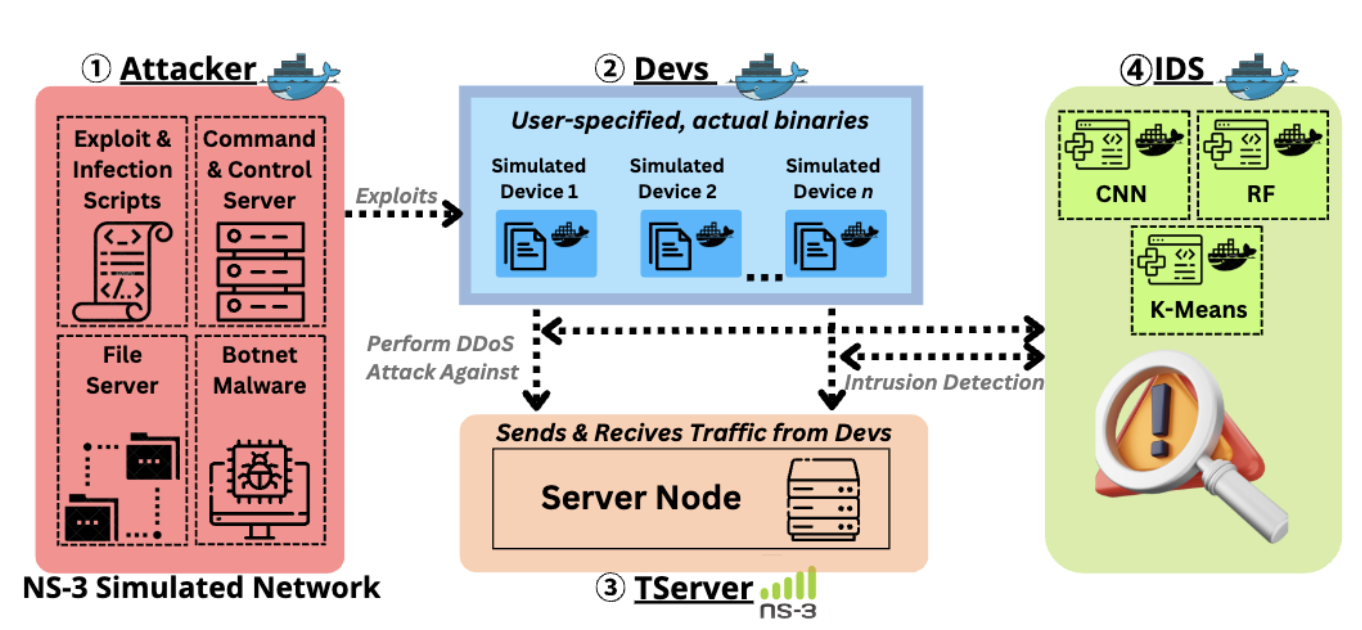
\includegraphics[scale= 0.6]{UNINA_MSc_Thesis_Project/img/chapterSimulatore/DDoShield.png}
  \caption{Architettura DDoShield}
\end{figure}


Questa architettura modulare consente di testare diverse configurazioni e scenari di attacco, rendendo DDoShield uno strumento flessibile e potente per la ricerca nel campo della sicurezza IoT.

Infine, oltre alla simulazione degli attacchi e alla valutazione delle prestazioni degli IDS in termini di accuratezza, DDoShield offre strumenti per misurare l'utilizzo delle risorse e la sostenibilità. Il tool è infatti in grado di rilevare metriche di performance degli IDS, come l'uso della CPU e della memoria, un aspetto cruciale quando si considera l'implementazione degli IDS in contesti IoT, dove i dispositivi hanno risorse limitate.

La valutazione delle prestazioni avviene in due fasi principali:
\begin{enumerate}
    \item \textbf{Fase di addestramento}: In questa fase, i modelli di machine learning sono addestrati su un dataset generato da DDoShield, che include sia traffico benigno che malevolo. I modelli vengono valutati in base a metriche come l'accuratezza, la precisione, il recall e l'F1-score. Durante questa fase, vengono anche misurate le risorse computazionali utilizzate per addestrare i modelli, in modo da determinare l'efficienza di ciascun algoritmo.
    \item \textbf{Fase di rilevamento in tempo reale}: Dopo l'addestramento, i modelli vengono utilizzati per rilevare attacchi in tempo reale durante la simulazione. Durante questa fase, DDoShield misura l'accuratezza del rilevamento, monitorando il tempo necessario per identificare un attacco e l'utilizzo delle risorse durante l'analisi del traffico di rete.
\end{enumerate}

Le metriche raccolte durante queste fasi offrono un quadro completo delle capacità del sistema IDS e permettono ai ricercatori di ottimizzare i modelli per ottenere il miglior compromesso tra accuratezza e utilizzo delle risorse. Per esempio, l'uso delle CNN può garantire una maggiore accuratezza nel rilevamento delle anomalie, ma al costo di un utilizzo di risorse computazionali più elevato rispetto ad altri modelli come il K-Means.
\cite{DDoShield}
\chapter{Il Dataset TON\_IoT}

Il dataset \textit{Ton\_IoT} rappresenta uno dei principali dataset utilizzati per l'addestramento e la valutazione dei modelli di \textit{Intrusion Detection System (IDS)}. È stato sviluppato dall'Università del New South Wales (UNSW) a Canberra ed è stato progettato per simulare scenari realistici di rete IoT. Il dataset è stato generato tramite un testbed complesso, che include vari livelli di interazione tra i dispositivi \textit{edge}, \textit{fog} e \textit{cloud}, emulando le comunicazioni tipiche dei sistemi IoT moderni.

Una delle ragioni della sua ampia diffusione è la sua natura estremamente eterogenea: \textit{Ton\_IoT} contiene dati di telemetria provenienti dai dispositivi IoT, dati estratti dai sistemi operativi (sia Windows che Linux) e dati relativi al traffico di rete. Questa caratteristica lo distingue da molti altri dataset nel campo della sicurezza informatica. Il nome stesso \textit{Ton\_IoT} deriva proprio dall'acronimo di \textit{Telemetry, Operating Systems, and Network Internet of Things}, riflettendo la varietà e la completezza delle fonti di dati incluse. \cite{Ton_IoT}

\section{Architettura del dataset}

L'architettura del dataset \textit{Ton\_IoT} è stata sviluppata per rappresentare una rete IoT complessa, distribuita su tre livelli principali: \textbf{edge}, \textbf{fog} e \textbf{cloud}. Questa struttura è stata implementata utilizzando tecnologie avanzate come \textit{Software-Defined Networking (SDN)}, \textit{Network Function Virtualization (NFV)} e \textit{Service Orchestration (SO)}.

\begin{itemize}
    \item \textbf{Livello Edge}: Questo livello è composto da dispositivi fisici IoT/IIoT che eseguono operazioni di rete, raccolgono dati sensoriali e comunicano con lo strato fog e cloud. Dispositivi come sensori per il monitoraggio ambientale, smart TVs e smartphones sono gestiti da gateway locali che indirizzano i dati verso lo strato fog.
    
    \item \textbf{Livello Fog}: Il livello fog integra la virtualizzazione delle funzioni di rete, utilizzando macchine virtuali (VMs) per l'analisi dei dati vicino alla sorgente. In questo contesto, le macchine virtuali distribuiscono i carichi di lavoro, eseguendo analisi preliminari e riducendo la latenza e la dipendenza dal cloud. La piattaforma VMware NSX è stata utilizzata per gestire le comunicazioni e la segmentazione della rete tra i vari livelli.
    
    \item \textbf{Livello Cloud}: Il livello cloud include servizi online, come il monitoraggio remoto dei dati e l'analisi approfondita del traffico di rete e dei dati IoT. Questo strato è responsabile dell'elaborazione di grandi volumi di dati provenienti dagli strati edge e fog. Servizi cloud come Microsoft Azure o AWS sono stati utilizzati per immagazzinare e processare i dati raccolti.
\end{itemize}

\begin{figure}[htbp]
\centering
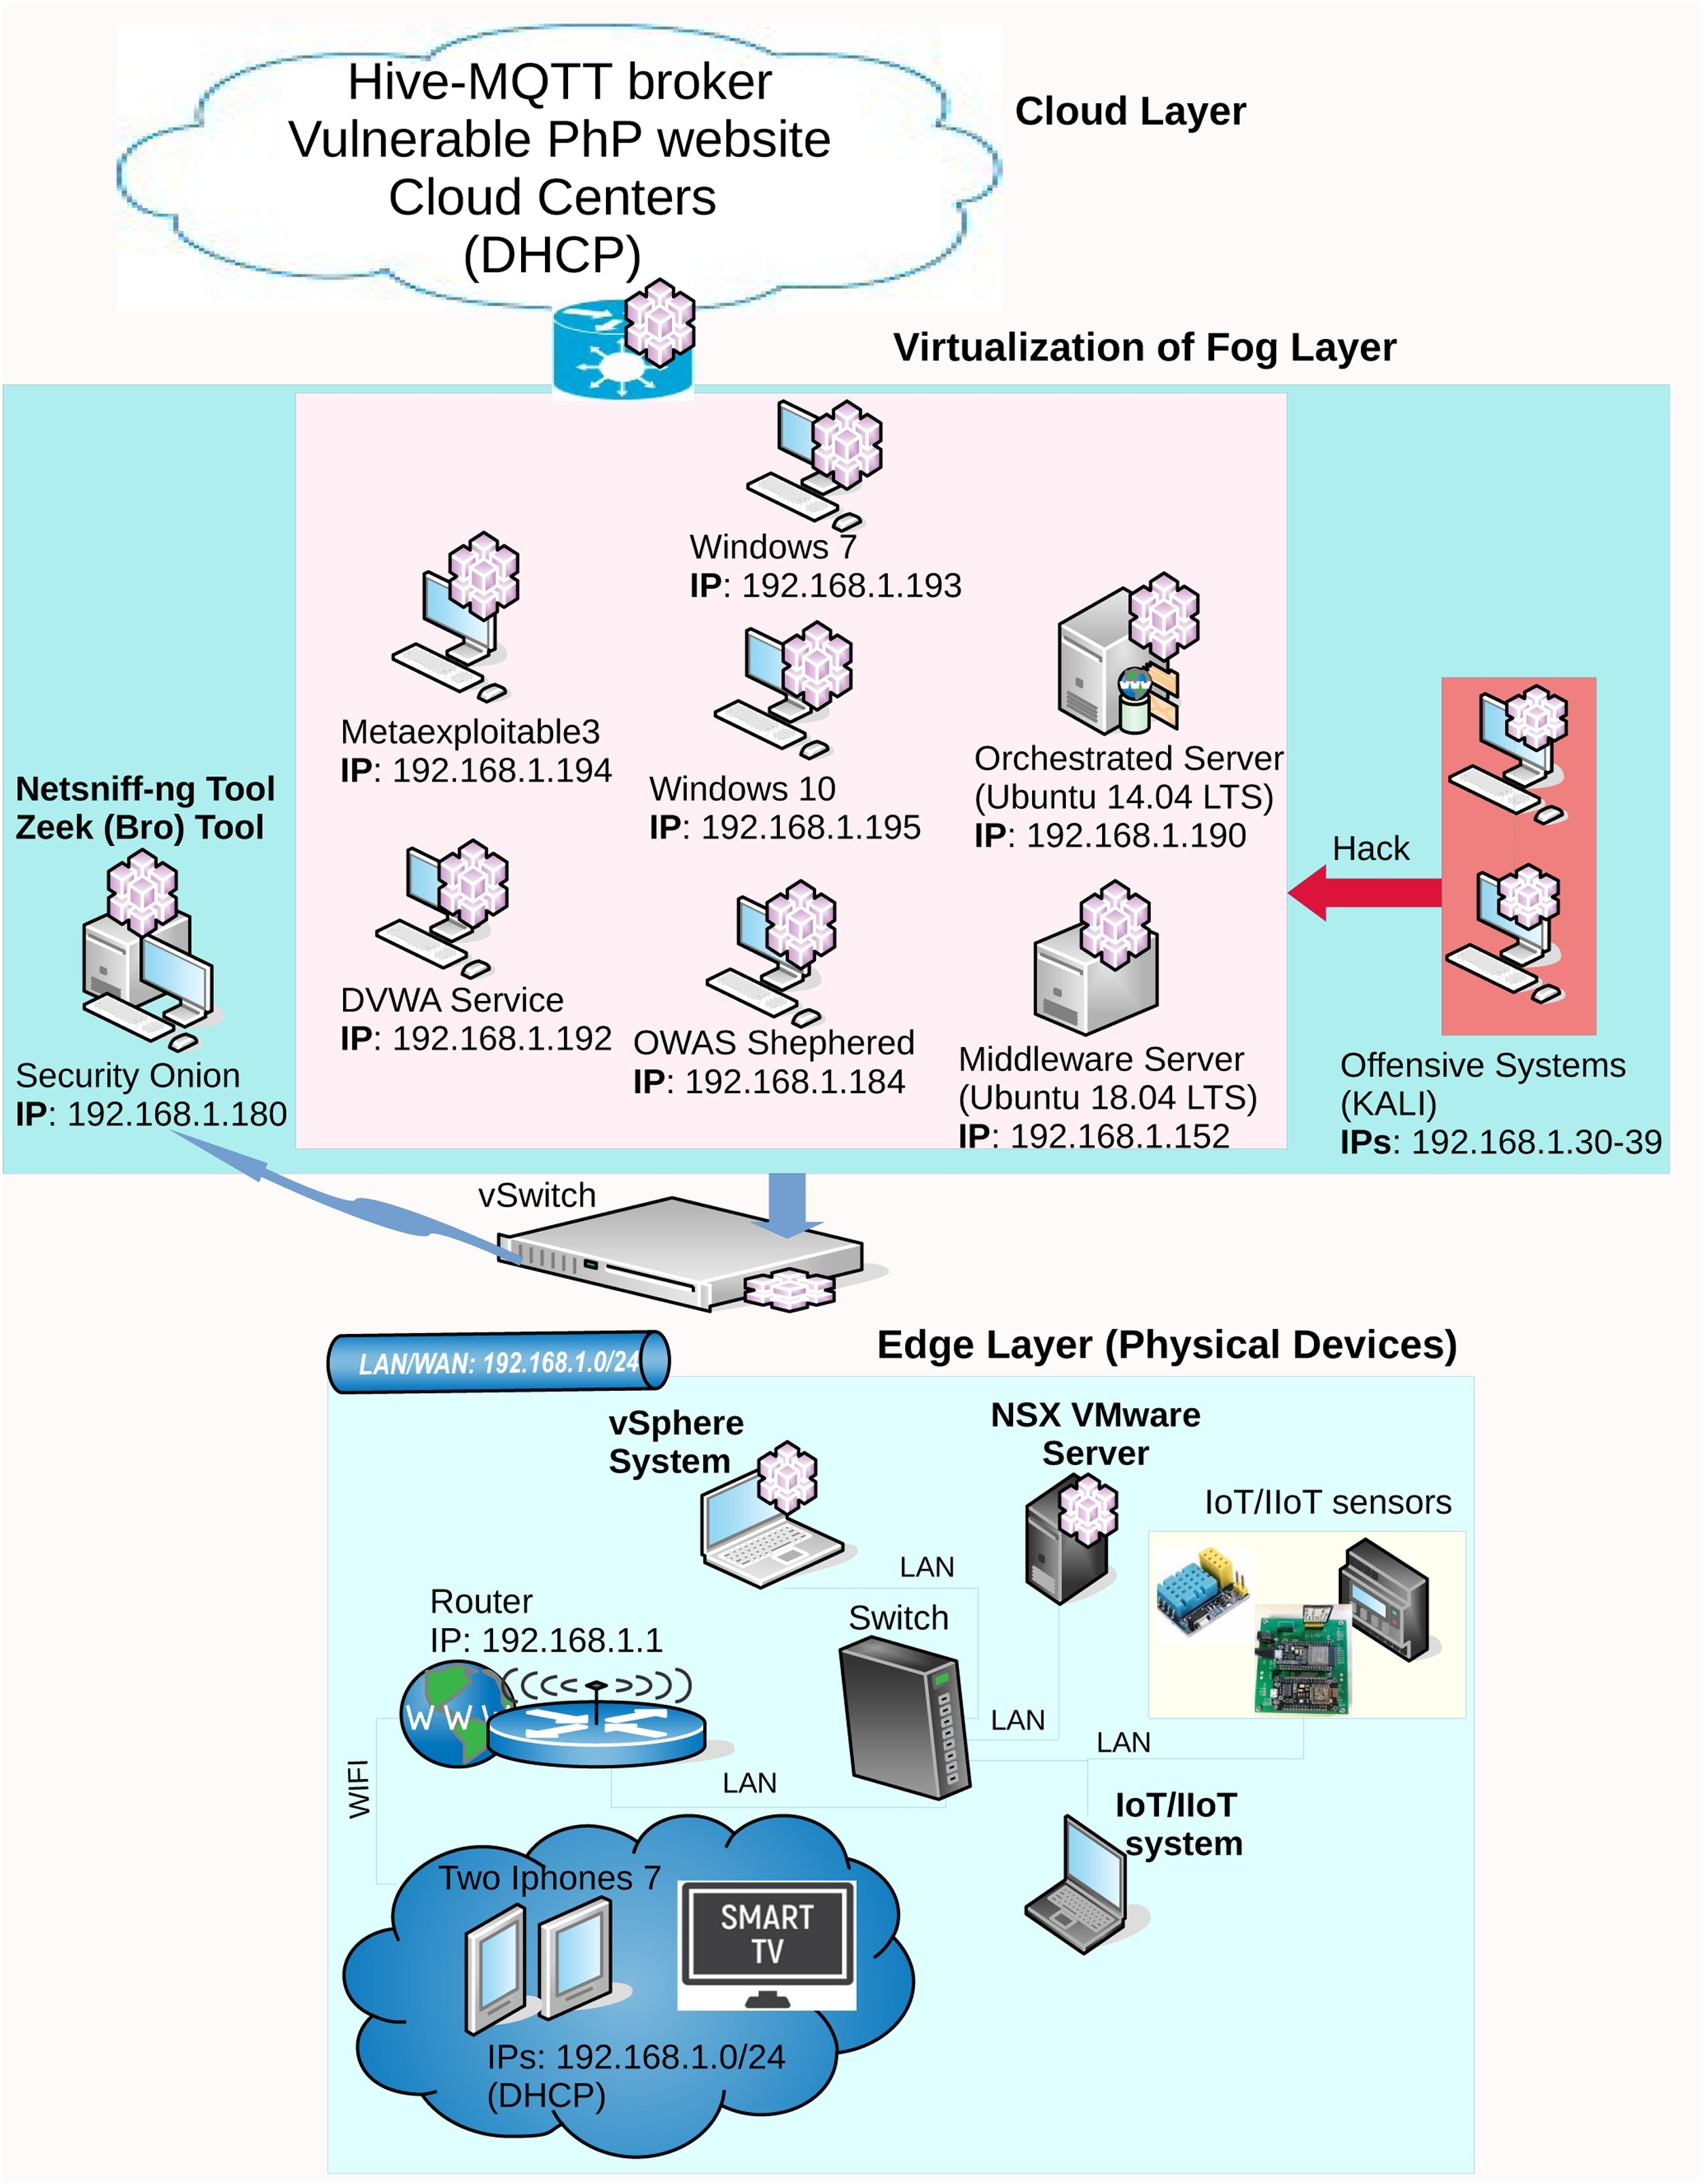
\includegraphics[scale= 0.7]{UNINA_MSc_Thesis_Project/img/Ton_Architecture.jpg}
  \caption{Architettura Ton IoT Dataset}
\end{figure}



\section{Tecnologie di supporto}

Le tecnologie alla base di questo testbed sono fondamentali per la flessibilità e la dinamicità delle interazioni tra i vari livelli:

\begin{itemize}
    \item \textbf{SDN (Software-Defined Networking)}: Consente di configurare in modo dinamico la rete tramite la programmabilità. Questa tecnologia è implementata tramite la piattaforma NSX-VMware, che permette di creare reti virtuali sovrapposte con funzionalità equivalenti a quelle fisiche.
    
    \item \textbf{NFV (Network Function Virtualization)}: Riduce la necessità di hardware specializzato sostituendo dispositivi fisici con funzioni di rete basate su software, eseguite come macchine virtuali. In questo modo, è possibile implementare scenari di attacco e normali all'interno del testbed.
    
    \item \textbf{SO (Service Orchestration)}: Gestisce l'orchestrazione dei servizi di rete, consentendo la distribuzione automatica delle risorse tra i vari livelli. L'integrazione di SO migliora l'efficienza operativa e garantisce la gestione dinamica dei flussi di dati tra edge, fog e cloud.
\end{itemize}

Questa architettura consente di raccogliere dati da diverse fonti eterogenee e offre un ambiente flessibile e realistico per valutare la capacità degli \textit{Intrusion Detection Systems (IDS)} di rilevare attacchi in ambienti distribuiti.

\section{Scenari di Attacco e Normali}

Il dataset \textit{Ton\_IoT} include sia traffico benigno che scenari di attacco. Gli scenari normali sono stati generati attraverso operazioni legittime che coinvolgono servizi IoT/IIoT come FTP, DNS e HTTP, simulati nel testbed. Gli scenari di attacco includono nove famiglie di attacchi: \textit{Denial of Service (DoS)}, \textit{Distributed Denial of Service (DDoS)}, \textit{injection}, \textit{Man-in-the-Middle (MITM)}, \textit{password cracking}, \textit{ransomware}, \textit{scanning}, \textit{XSS} e \textit{backdoor}. Ogni attacco è stato lanciato contro vulnerabilità specifiche nei servizi IoT/IIoT o nei sistemi operativi ospitati.

\section{Motivazione per l'Uso del Ton\_IoT nella Tesi}

Il dataset \textit{Ton\_IoT} è stato scelto per questo lavoro di tesi per la sua capacità di rappresentare scenari realistici che coinvolgono interazioni tra dispositivi IoT/IIoT e sistemi di rete distribuiti. Una delle caratteristiche principali del dataset è la raccolta di dati eterogenei da quattro fonti: traffico di rete, telemetria dei dispositivi IoT, tracce di audit di sistemi operativi (Windows e Linux), e dati di attacco generati da scenari di hacking simulati. Questo lo rende particolarmente adatto per valutare l'efficacia di sistemi di \textit{Intrusion Detection System (IDS)} basati su tecniche di \textit{machine learning} in ambienti IoT, che rappresentano il focus centrale di questo lavoro di tesi.

Inoltre, la struttura del dataset permette di esplorare come differenti livelli di simulazione e attacchi distribuiti possano influenzare la capacità di generalizzazione degli \textit{IDS}.

\section{Caratteristiche Principali del Dataset}

Il dataset è suddiviso in vari file in formato CSV e pcap che contengono i dati etichettati relativi agli attacchi e ai normali scenari di rete. Ogni file contiene 44 attributi, che descrivono varie caratteristiche del traffico di rete e delle operazioni di sistema. Sono inoltre presenti etichette che indicano se il record rappresenta un comportamento normale o un attacco, e in caso di attacco, il tipo specifico di attacco. Questi dati sono stati utilizzati per addestrare e testare diversi modelli di apprendimento automatico durante gli esperimenti di questa tesi.


\chapter{La Data Augmentation}

La Data Augmentation è una tecnica fondamentale nel campo dell’apprendimento automatico, utilizzata principalmente per aumentare la quantità e la diversità dei dati di addestramento, migliorando così le prestazioni dei modelli di machine learning. In particolare, è ampiamente adottata nelle applicazioni che lavorano con grandi quantità di dati, come nel riconoscimento delle immagini, l'elaborazione del linguaggio naturale e, più recentemente, nell’ambito della sicurezza informatica e dell'Internet of Things (IoT). Nei prossimi paragrafi verrà fornita una panoramica completa della Data Augmentation, illustrando le tecniche più comuni, i vantaggi e gli svantaggi e i principali casi d'uso.

\section{Cos'è la Data Augmentation}

La Data Augmentation consiste nell'applicare una serie di trasformazioni ai dati esistenti per generare nuove istanze da utilizzare per l'addestramento di un modello. Queste trasformazioni possono essere di natura semplice, come rotazioni o traslazioni nel caso di immagini, oppure più complesse, come la generazione sintetica di nuovi campioni basati su tecniche di apprendimento. L'obiettivo principale della Data Augmentation è quello di ridurre l'overfitting migliorando la generalizzazione del modello, senza la necessità di raccogliere ulteriori dati, che potrebbe essere un processo costoso e complesso oltre che spesso non applicabile.

Esistono diverse tecniche di Data Augmentation, alcune delle quali sono specifiche per determinati tipi di dati (come immagini o testo), mentre altre sono più generiche e applicabili a vari domini. La scelta delle trasformazioni dipende dal tipo di dati e dal problema da risolvere.\cite{dataAugmentation}

\section{Tecniche comuni di Data Augmentation}

Le tecniche di Data Augmentation possono variare considerevolmente in base al tipo di dati e all’applicazione specifica. Di seguito vengono elencate alcune delle tecniche più comuni.

\subsection{Per dati immagine}
Per i dati immagine, la Data Augmentation si basa principalmente su trasformazioni geometriche e modifiche ai pixel, che possono essere applicate a ogni immagine nel dataset. Tra le trasformazioni più utilizzate troviamo:

\begin{itemize}
    \item \textbf{Rotazione}: Rotare l'immagine di un certo angolo, generalmente casuale, permette di introdurre variabilità nella posizione degli oggetti, migliorando la robustezza del modello a diverse orientazioni.
    \item \textbf{Riflesso orizzontale o verticale}: Consiste nel riflettere l'immagine lungo l'asse orizzontale o verticale, fornendo una vista speculare dell'immagine originale. Questa tecnica è particolarmente utile nel riconoscimento di oggetti o volti.
    \item \textbf{Ridimensionamento e traslazione}: Modificare la scala o la posizione degli oggetti presenti nelle immagini per rendere il modello più resiliente alle variazioni nelle dimensioni e nella posizione degli oggetti.
    \item \textbf{Distorsioni di colore e illuminazione}: Modificare la saturazione, il contrasto e la luminosità delle immagini per simulare diverse condizioni di illuminazione.
    \item \textbf{Rumore aggiunto}: Aggiungere rumore casuale ai pixel per migliorare la capacità del modello di gestire dati rumorosi o imperfetti.
\end{itemize}

\subsection{Per dati testuali}
Nel caso dei dati testuali, la Data Augmentation presenta sfide diverse, poiché il linguaggio naturale è sensibile alle variazioni nel significato delle parole. Tuttavia, ci sono tecniche utili, tra cui:

\begin{itemize}
    \item \textbf{Sostituzione sinonimica}: Consiste nel sostituire alcune parole con i loro sinonimi, mantenendo invariato il significato complessivo della frase, ma introducendo una nuova rappresentazione.
    \item \textbf{Cancellazione di parole}: Rimuovere casualmente alcune parole non critiche all'interno di una frase per creare varianti che mantengano il significato generale.
    \item \textbf{Riordino delle parole}: Cambiare l’ordine di alcune parole, specialmente in frasi dove il significato non dipende strettamente dalla sequenza precisa.
    \item \textbf{Traduzione inversa}: Tradurre un testo in una lingua diversa e poi riconvertirlo alla lingua originale, creando nuove espressioni mantenendo intatto il significato.
\end{itemize}

\subsection{Per dati tabulari}
Nel caso dei dati strutturati, come quelli presenti in tabelle, la Data Augmentation si concentra più sulla creazione di nuovi esempi sintetici attraverso tecniche avanzate, come:

\begin{itemize}
    \item \textbf{Jittering}: Aggiungere rumore casuale a valori numerici, specialmente nei dati continui.
    \item \textbf{Synthetic Minority Over-sampling Technique (SMOTE)}: Un algoritmo che genera nuove istanze sintetiche per bilanciare le classi minoritarie all'interno di un dataset.
    \item \textbf{Copia e interpolazione}: Per alcune categorie di dati, può essere utile duplicare esempi o crearne di nuovi attraverso interpolazione tra i dati esistenti.
\end{itemize}

\section{Benefici della Data Augmentation}

L'adozione della Data Augmentation offre numerosi vantaggi, soprattutto in contesti in cui la raccolta di dati è costosa o limitata. Ecco alcuni dei principali benefici che derivano dall'uso di questa tecnica.

\subsection{Riduzione dell'overfitting}

Uno dei problemi principali quando si lavora con dataset di piccole dimensioni è il rischio di overfitting. Ciò accade quando un modello apprende troppo bene i dettagli e il rumore presenti nei dati di addestramento, a scapito della sua capacità di generalizzare a nuovi dati. La Data Augmentation mitiga questo problema generando varianti del dataset originale, aumentando la variabilità dei dati e costringendo il modello ad apprendere caratteristiche generali piuttosto che dettagli specifici.

\subsection{Miglioramento delle prestazioni del modello}

Aumentare la quantità di dati disponibili per l'addestramento di un modello può migliorare notevolmente le sue prestazioni. La Data Augmentation fornisce nuovi esempi senza dover raccogliere o etichettare manualmente nuovi dati, riducendo i costi associati alla creazione di dataset più grandi. Questo è particolarmente utile in applicazioni come il riconoscimento delle immagini o l'elaborazione del linguaggio naturale, dove la raccolta di nuovi dati è spesso laboriosa.

\subsection{Robustezza ai cambiamenti e alle variazioni}

Un altro beneficio chiave della Data Augmentation è la capacità di rendere i modelli più robusti alle variazioni nei dati di input. Ad esempio, nei modelli di riconoscimento delle immagini, le tecniche di trasformazione (come rotazione, traslazione o ridimensionamento) preparano il modello a riconoscere oggetti indipendentemente dalla loro posizione o orientamento. Nel contesto dell'IoT, questo si traduce in modelli capaci di adattarsi meglio a condizioni variabili e a dispositivi eterogenei.

\subsection{Migliore generalizzazione}

Grazie alla maggiore variabilità introdotta nei dati di addestramento, i modelli addestrati con Data Augmentation tendono a generalizzare meglio. Questo significa che i modelli saranno in grado di fare previsioni più accurate su dati non visti durante l'addestramento. La Data Augmentation è particolarmente utile quando si hanno a disposizione pochi dati e si desidera migliorare la capacità del modello di riconoscere pattern nascosti nei nuovi dati.

\subsection{Affrontare il class imbalance}

In molti contesti di machine learning, specialmente nell'IoT o nella sicurezza informatica, i dataset possono essere sbilanciati, con poche istanze appartenenti a una classe minoritaria. La Data Augmentation consente di generare nuovi esempi per bilanciare le classi, migliorando così la capacità del modello di apprendere dalle classi meno rappresentate e di ridurre il rischio di bias.

\section{Contro della Data Augmentation}

Nonostante i numerosi benefici, la Data Augmentation presenta anche alcune limitazioni e svantaggi che devono essere presi in considerazione prima della sua implementazione.

\subsection{Possibile aggiunta di rumore ai dati}

Un problema comune con la Data Augmentation è che, se non eseguita correttamente, può introdurre rumore o distorsioni nei dati di addestramento. Ad esempio, in un'applicazione di riconoscimento delle immagini, se le trasformazioni applicate sono troppo estreme (come un'eccessiva rotazione o ridimensionamento), si rischia di alterare l'immagine in modo tale che non rappresenti più l'oggetto originale. Questo può portare a una riduzione delle prestazioni del modello, poiché il modello apprende caratteristiche fuorvianti.

\subsection{Crescita del tempo di addestramento}

Generare nuovi dati attraverso la Data Augmentation può aumentare significativamente il tempo di addestramento di un modello. L'aggiunta di nuovi esempi al dataset richiede più tempo per completare ogni epoca di addestramento, soprattutto se il dataset diventa molto grande. Sebbene ciò possa migliorare le prestazioni del modello, può anche richiedere risorse computazionali aggiuntive e aumentare i costi associati all'addestramento del modello.

\subsection{Sovraccarico computazionale}

Alcune tecniche di Data Augmentation, come la generazione sintetica di nuovi esempi tramite reti neurali generative (GANs) o altre tecniche avanzate, possono richiedere risorse computazionali significative. In contesti come l'IoT, dove i dispositivi hanno capacità di calcolo limitate, questo può rappresentare un ostacolo all'implementazione della Data Augmentation direttamente sui dispositivi.

\subsection{Rischio di overfitting sulla Data Augmentation}

In alcuni casi, se la Data Augmentation non è ben progettata, può portare a una sorta di overfitting sui dati aumentati. Questo avviene quando il modello apprende troppo dalle trasformazioni generate e diventa meno capace di generalizzare su dati reali non trasformati. È quindi importante scegliere tecniche di Data Augmentation che riflettano il più possibile le variazioni reali dei dati.

\subsection{Difficoltà nell’applicazione a dati complessi}

Infine, applicare la Data Augmentation a dati complessi, come quelli testuali o tabulari, può risultare problematico. Mentre è relativamente semplice applicare trasformazioni geometriche a immagini, le operazioni sui dati testuali devono preservare il significato delle frasi, e alterazioni troppo drastiche possono introdurre errori o distorsioni nel significato. Lo stesso vale per i dati tabulari, dove modifiche non appropriate possono alterare i rapporti logici tra le variabili. \cite{consDataAugmentation}

\chapter{Metodologia e strumenti utilizzati}
Nel capitolo dedicato alla metodologia e agli strumenti utilizzati, vengono delineati i principi fondamentali che guidano la ricerca, nonché le tecniche e le tecnologie impiegate per raggiungere gli obiettivi prefissati. Questo capitolo fornisce una panoramica delle scelte metodologiche adottate, con particolare attenzione all'approccio di Data Augmentation e all'impiego di dati simulati per ottimizzare l'addestramento dei sistemi di rilevamento delle intrusioni (IDS). Verranno descritti i modelli e gli algoritmi di machine learning selezionati, oltre agli strumenti software utilizzati per l'analisi dei dati e la valutazione delle prestazioni dei modelli. Questa sezione è fondamentale per comprendere il contesto in cui si inserisce la ricerca e per garantire la riproducibilità dei risultati ottenuti.

\section{Workflow}

In questa sezione, verranno chiariti l'obiettivo della tesi e il flusso di lavoro seguito per raggiungerlo. L'obiettivo principale è valutare come variano le performance dell'IDS adottando un approccio di Data Augmentation. In particolare, si vuole esaminare l'impatto di questa tecnica nel migliorare la capacità del sistema di rilevare anomalie e attacchi in contesti IoT. Il workflow descritto in figura fornisce una panoramica dettagliata delle fasi seguite durante l'intero processo. Di seguito, descriviamo le varie fasi operative:

\begin{figure}[htbp]
\centering
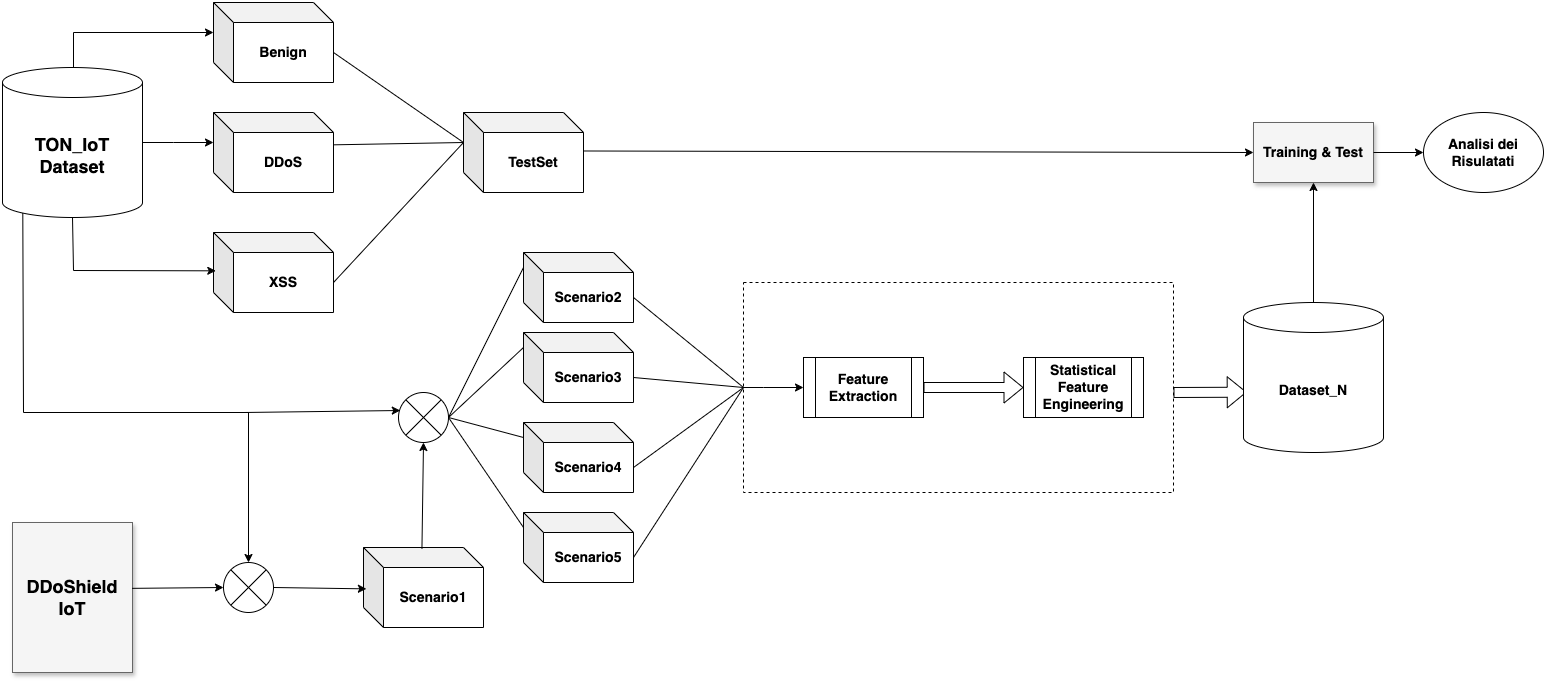
\includegraphics[scale= 0.27]{UNINA_MSc_Thesis_Project/img/chapterMetodologia/Workflow_Bold_XXL.png}
  \caption{Workflow seguito}
\end{figure}


\begin{itemize}
    \item \textbf{Definizione e creazione di diversi scenari}: Per rappresentare una varietà di situazioni e contesti di rete, sono stati creati più scenari che simulano condizioni reali, inclusi diversi tipi di traffico di rete e differenti intensità di attacco DDoS. Questi scenari permettono di valutare le prestazioni dell'IDS in ambienti eterogenei.
    
    \item \textbf{Raccolta dei dati}: I dati sono stati acquisiti attraverso il tool \texttt{tcpdump}, che fa parte della suite Wireshark. Questo strumento ha permesso di catturare il traffico di rete sia benigno che malevolo, generando un dataset realistico per l'addestramento e la valutazione dei modelli di rilevamento delle intrusioni.
    
    \item \textbf{Estrazione delle feature di interesse}: Dopo la raccolta dei dati, è stato effettuato un processo di estrazione delle feature che ci interessano maggiormente per il rilevamento delle anomalie. Queste feature includono parametri relativi al traffico, come la dimensione dei pacchetti, il tempo di trasmissione e il numero di pacchetti inviati in una finestra temporale definita.
    
    \item \textbf{Processo di feature engineering}: Successivamente, si è proceduto con un processo di feature engineering per migliorare la qualità dei dati e ottimizzare le feature utilizzate per l'addestramento. Questo passaggio è fondamentale per aumentare l'efficacia del modello e ridurre l'overfitting, migliorando così la sua capacità di generalizzare su nuovi dati.
    
    \item \textbf{Creazione di un test set}: È stato creato un test set separato, composto da dati non utilizzati nella fase di addestramento, per valutare in maniera imparziale le performance dei modelli di rilevamento. Il test set include sia traffico benigno che attacchi simulati, con lo scopo di testare la capacità dell'IDS di distinguere tra i due.
    
    \item \textbf{Analisi e discussione dei risultati}: Una volta addestrati e testati i modelli, è stata eseguita un'analisi approfondita dei risultati. Questa fase include la valutazione delle metriche di performance (come accuratezza, precisione, recall e F1-score), e la discussione sull'impatto della Data Augmentation sulle prestazioni dell'IDS, mettendo in evidenza i vantaggi e le limitazioni della tecnica adottata.
\end{itemize}

Il workflow descritto assicura una metodologia rigorosa e riproducibile per valutare l'efficacia dell'uso della Data Augmentation nel migliorare le performance degli IDS in ambienti IoT. Ogni fase è stata eseguita con l'obiettivo di massimizzare la generalizzazione del modello e di ottenere un quadro dettagliato delle sue capacità in scenari complessi e variabili.

\section{Scenari Riprodotti}
I dataset utilizzati in questo lavoro sono stati costruiti con l'obiettivo di fornire una varietà di scenari di traffico di rete, con diverse distribuzioni di attacchi e protocolli, al fine di testare e addestrare modelli di rilevamento delle intrusioni. I dataset sono suddivisi in cinque diverse configurazioni, ciascuna caratterizzata da una combinazione specifica di traffico benigno e maligno, con l'aggiunta o la rimozione del contributo di un simulatore che verrà introdotto in seguito. Questa diversificazione consente di analizzare l'efficacia degli \textit{IDS} su scenari realistici e variabili, riflettendo le condizioni tipiche delle reti IoT.

\textbf{Dataset 1}: Il primo dataset rappresenta la base su cui sono stati costruiti tutti gli altri. Esso è costituito da una porzione del traffico benigno del \textit{TON\_IoT dataset} combinato con il traffico generato dal simulatore \textit{DDoShield}, che include sia traffico benigno che maligno. Questo dataset contiene un totale di circa 1.670.000 pacchetti, con una distribuzione di circa 57.34\% di pacchetti benigni e 42.66\% di pacchetti maligni appartenenti ad attacchi DDoS. A partire da questo dataset, frazionando il traffico maligno saranno generati gli altri scenari.

\begin{figure}[htbp]
\centering
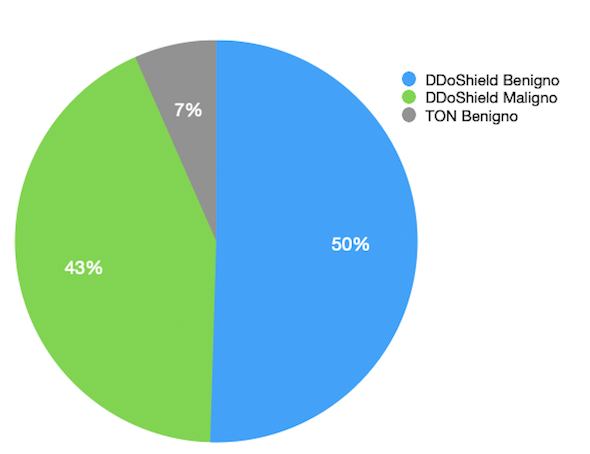
\includegraphics[scale= 0.8]{UNINA_MSc_Thesis_Project/img/chapterRisulati/composizione_DATASET_1 centrata.png}
  \caption{Composizione Dataset 1}
\end{figure}

\textbf{Dataset 2}: Questo dataset è stato creato mantenendo invariato il traffico benigno del \textit{Dataset 1} e frazionando il traffico maligno del \textit{DDoShield}. La suddivisione del traffico maligno è stata fatta in modo equo, con il 50\% di pacchetti provenienti dal \textit{DDoShield} e il 50\% provenienti dal \textit{TON\_IoT}, limitati all'attacco \textit{DDoS}. Questo dataset è particolarmente utile per testare la capacità degli \textit{IDS} di rilevare attacchi \textit{DDoS} distribuiti su diverse fonti.

\begin{figure}[htbp]
\centering
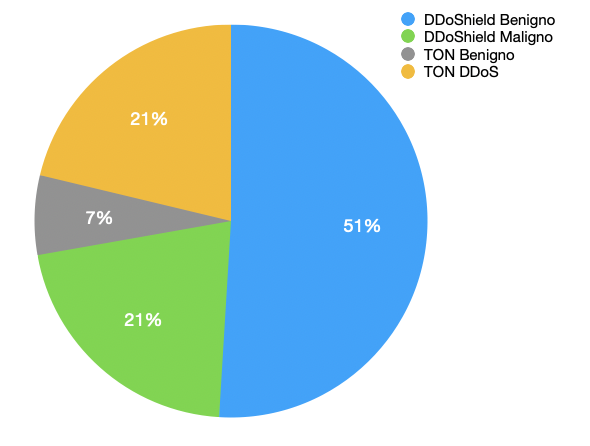
\includegraphics[scale= 0.8]{UNINA_MSc_Thesis_Project/img/chapterRisulati/composizione_DATASET_2.png}
  \caption{Composizione Dataset 2}
\end{figure}

\textbf{Dataset 3}: Il terzo dataset segue una logica simile al \textit{Dataset 2}, ma con una diversa distribuzione del traffico maligno: il 70\% del traffico maligno proviene dal \textit{DDoShield}, mentre il restante 30\% dal \textit{TON\_IoT} con attacchi \textit{DDoS}. Questa configurazione aumenta l'enfasi sugli attacchi simulati rispetto a quelli reali, creando uno scenario più complesso in cui testare la capacità di generalizzazione degli \textit{IDS} di fronte a differenti fonti di attacco.

\begin{figure}[htbp]
\centering
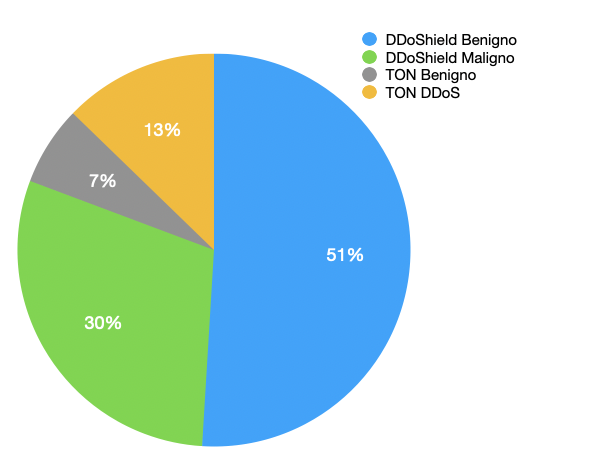
\includegraphics[scale= 0.8]{UNINA_MSc_Thesis_Project/img/chapterRisulati/composizione_DATASET_3.png}
  \caption{Composizione Dataset 3}
\end{figure}

\textbf{Dataset 4}: Questo dataset inverte la proporzione del traffico maligno rispetto al \textit{Dataset 3}, con il 30\% proveniente dal \textit{DDoShield} e il 70\% dal \textit{TON\_IoT} (sempre con attacchi \textit{DDoS}). Questa configurazione è particolarmente importante per testare la robustezza degli \textit{IDS} nei confronti di attacchi reali con una bassa interferenza di dati simulati. La prevalenza di traffico \textit{DDoS} reale rende questo dataset utile per l'analisi della capacità del sistema di rilevare minacce realistiche in ambienti IoT.

\begin{figure}[htbp]
\centering
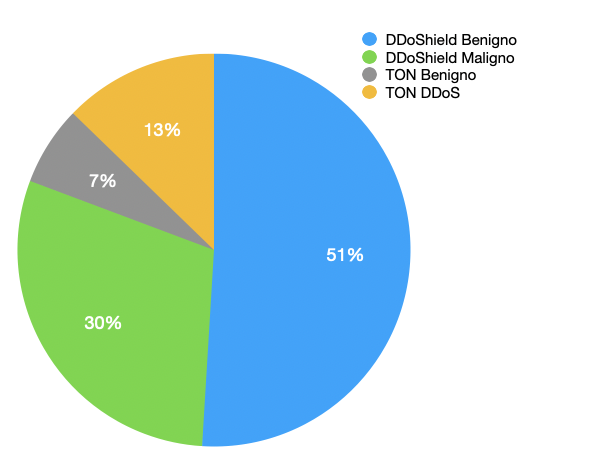
\includegraphics[scale= 0.8]{UNINA_MSc_Thesis_Project/img/chapterRisulati/composizione_DATASET_4.png}
  \caption{Composizione Dataset 4}
\end{figure}

\textbf{Dataset 5}: Questo dataset introduce una maggiore complessità includendo non solo attacchi \textit{DDoS}, ma anche attacchi \textit{XSS} (\textit{Cross-Site Scripting}) provenienti dal \textit{TON\_IoT dataset}. In questa configurazione, il traffico maligno è suddiviso equamente tra il 50\% di pacchetti provenienti dal \textit{DDoShield} e il 50\% proveniente dal \textit{TON\_IoT}, ulteriormente frazionato in 25\% \textit{DDoS} e 25\% \textit{XSS}. Questo dataset rappresenta uno scenario multi-attacco complesso, che mette alla prova la capacità degli \textit{IDS} di gestire simultaneamente più tipologie di minacce, rendendo particolarmente interessante l'analisi della loro capacità di distinguere fra attacchi di natura diversa.

\begin{figure}[htbp]
\centering
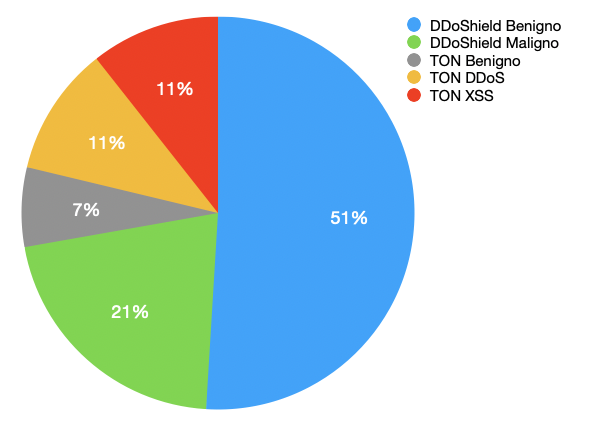
\includegraphics[scale= 0.8]{UNINA_MSc_Thesis_Project/img/chapterRisulati/composizione_DATASET_5.png}
  \caption{Composizione Dataset 5}
\end{figure}

La scelta delle percentuali è finalizzata a riprodurre condizioni diverse e quindi scenari favorevoli e sfavoreli con lo scopo ultimo di isolare l'impatto del simulatore e trovare il giusto compromesso per l'addestramento degli IDS.

Per valutare gli scenari descritti, è stato creato un \textit{test set} della dimensione pari al 20\% dei \textit{dataset}, ottenuto tramite un campionamento casuale di pacchetti non presenti nel set di \textit{train} estratti dal \textit{TON\_IoT dataset}. La scelta di utilizzare il 20\% deriva dalla necessità di avere una porzione di dati sufficientemente rappresentativa per testare il modello, senza però compromettere la quantità di dati disponibili per l'addestramento. Questo rapporto tra \textit{train} e \textit{test} è comunemente adottato in ambito di machine learning per garantire che il modello sia esposto a una varietà adeguata di pattern durante la fase di addestramento, mantenendo al contempo una solida base di dati indipendenti per la valutazione delle prestazioni.

Inoltre, la selezione casuale garantisce che il \textit{test set} contenga una distribuzione rappresentativa sia di traffico benigno che di traffico maligno, minimizzando così il rischio di bias e garantendo una valutazione più robusta del modello. Con un \textit{test set} ben bilanciato e di dimensioni adeguate, è possibile ottenere una stima più accurata della generalizzazione del modello a nuovi dati non visti, condizione essenziale per il deployment in scenari reali, come la protezione di reti IoT. \cite{DeepLearning}

\section{Tecniche di rilevamento delle anomalie}
Negli IDS basati su un approccio \textit{anomaly-based}, come abbiamo visto nel capitolo precedente, la vasta quantità di dati da analizzare può rendere complesso individuare anomalie in tempo reale. Di conseguenza, la scelta della tecnica utilizzata per il rilevamento assume un'importanza cruciale. Nei paragrafi seguenti, forniremo una panoramica di queste tecniche, evidenziando i vantaggi e le limitazioni di ciascuna.
%TODO: Forse questo pezzettino è da aggiustare o comunque riformulare il concetto, ASPETTA di avere più chiaro l'ordine del capitolo 
Abbiamo già discusso le principali differenze tra un approccio basato su firme e uno basato sul rilevamento delle anomalie. Ora possiamo approfondire le possibili soluzioni implementative per quest'ultimo approccio, che mira a individuare comportamenti anomali rispetto al normale funzionamento del sistema. Questi metodi, pur avendo vantaggi significativi, richiedono una gestione attenta del modello e dei dati, poiché un numero elevato di falsi positivi potrebbe rendere il sistema meno efficace. Esploriamo di seguito alcune delle principali tecniche adottate nell'ambito del rilevamento delle anomalie:

\begin{longtable}{|p{3cm}|p{3cm}|p{4cm}|p{4cm}|}
\hline
\textbf{Tecniche} & \textbf{Modelli} & \textbf{Vantaggi} & \textbf{Svantaggi} \\
\hline
\endfirsthead % Intestazione della prima pagina
\hline
\textbf{Tecniche} & \textbf{Modelli} & \textbf{Vantaggi} & \textbf{Svantaggi} \\
\hline
\endhead % Intestazione delle pagine successive

\multirow{4}{3cm}{\raggedright \textbf{Basato su firme}} 
 & • Confronto di pattern & • Alta accuratezza per attacchi noti & • Incapacità di rilevare attacchi nuovi o sconosciuti \\
 & • Analisi dei protocolli & • Basso tasso di falsi positivi & • Dipendenza dagli aggiornamenti delle firme \\
 & • Ispezione dei contenuti & • Facile da implementare & • Mancanza di flessibilità \\
 & • Analisi dei log & • Basso overhead computazionale & • Copertura limitata \\
\hline
\multirow{3}{3cm}{\raggedright \textbf{Modelli Statistici}} 
 & • Rilevamento di anomalie & • Metodo consolidato con una solida base teorica & • Capacità limitata di rilevare anomalie complesse o sofisticate \\
 & • Analisi delle serie temporali & • Adatto per il rilevamento di anomalie semplici & • Sensibilità alla distribuzione dei dati e alle assunzioni \\
 & • Modellazione statistica & • Risultati interpretabili & • Difficoltà nella gestione di dati ad alta dimensionalità \\
\hline
\multirow{4}{3cm}{\raggedright \textbf{Machine Learning}} 
 & • Clustering & • Capacità di gestire pattern complessi e non lineari & • Necessità di grandi set di dati etichettati per l'addestramento \\
 & • Classificazione & • Efficace per identificare anomalie sottili & • Possibile overfitting se non ottimizzato correttamente \\
 & • Reti neurali & • Adattabilità a ambienti mutevoli & • Complessità computazionale elevata per algoritmi complessi \\
 &  & • Può apprendere da dati non etichettati o parzialmente etichettati & • La natura "black-box" può limitare l'interpretabilità \\
\hline
\multirow{4}{3cm}{\raggedright \textbf{Approcci Ibridi}} 
 & • Modelli Statistici + Machine Learning & • Sfruttare i punti forti di entrambe le tecniche & • Aumenta la complessità del sistema e della sua integrazione \\
 &  & • Precisione ed affidabilità migliorate & • Risorse computazionali più elevate \\
 &  & • Maggiori capacità di gestire diverse anomalie &  \\
\hline
\caption{Confronto tra tecniche IDS, modelli, vantaggi e svantaggi}
\label{tab:confronto_ids}
\end{longtable}

\begin{itemize}
\item \textbf{Approccio statistico}: Questo metodo si basa su modelli matematici che analizzano il comportamento storico del sistema per stabilire una baseline, o comportamento normale. Le deviazioni significative da questa baseline vengono interpretate come potenziali anomalie. Gli approcci statistici possono includere tecniche come il calcolo della media, deviazione standard, analisi della varianza e regressione. Sebbene siano semplici da implementare, possono risultare inefficaci in ambienti dinamici dove il comportamento normale cambia frequentemente, portando a falsi positivi o falsi negativi.

\item \textbf{Approccio con tecniche di Machine Learning}: L'utilizzo di algoritmi di apprendimento automatico rappresenta una soluzione avanzata per il rilevamento delle anomalie. Attraverso l'addestramento su grandi quantità di dati storici, un modello di machine learning può apprendere a distinguere tra comportamenti normali e anomali. Gli algoritmi di apprendimento possono seguire due tipi di approccio: quello \textbf{supervisionato}, che include tecniche come le reti neurali o gli alberi decisionali, e richiede un dataset etichettato per l'addestramento; e quello \textbf{non supervisionato}, che comprende metodi come il clustering o gli autoencoder, i quali non necessitano di etichette e possono identificare anomalie senza una conoscenza preliminare.

Il primo approccio è particolarmente efficace per il rilevamento di anomalie già note, ma presenta limitazioni quando si tratta di individuare nuove anomalie. Al contrario, il secondo approccio offre maggiore flessibilità, ma la sua efficacia è strettamente legata alla qualità e alla quantità dei dati utilizzati per l'addestramento. In molti contesti applicativi, non c'è disponibilità di dati pre-etichettati, motivo per cui gli algoritmi di machine learning non supervisionati sono spesso preferiti.

\begin{figure}[htbp]
\centering
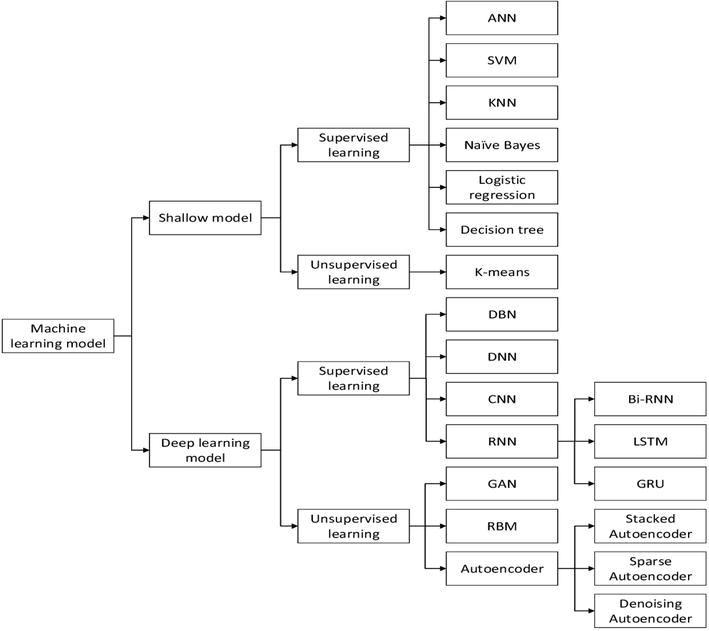
\includegraphics[scale= 0.9]{UNINA_MSc_Thesis_Project/img/chapterMetodologia/machineLearnin_models.png}
  \caption{Famiglie di Modelli di Machine Learning}
\end{figure}

\item \textbf{Approcci ibridi}: Gli approcci ibridi combinano tecniche statistiche e di machine learning per migliorare l'accuratezza e l'efficacia del rilevamento delle anomalie negli IDS. Sfruttando i punti di forza di entrambe le metodologie, i modelli ibridi offrono capacità di rilevamento più avanzate e complete. Ad esempio, un approccio ibrido può utilizzare tecniche statistiche per definire il comportamento di base del sistema e algoritmi di machine learning per classificare le istanze come normali o anomale. Questa combinazione permette di realizzare un sistema di rilevamento delle anomalie più completo e robusto. \cite{AnomalyDetection}
\end{itemize}

\section{Algoritmi Utilizzati per l'Addestramento}

In questa sezione vengono descritti gli algoritmi utilizzati per l'addestramento dei modelli di IDS: \textit{K-Means}, \textit{Random Forest (RF)} e \textit{Convolutional Neural Network (CNN)}. Questi algoritmi sono stati scelti per le loro capacità di gestire grandi quantità di dati e rilevare pattern complessi in contesti di sicurezza informatica.

\subsection{K-Means}

\textit{K-Means} è un algoritmo di clustering non supervisionato utilizzato per suddividere un insieme di dati in $k$ gruppi, dove ogni gruppo è rappresentato dal suo centroide. L'algoritmo funziona iterativamente per minimizzare la varianza interna ai cluster, cercando di assegnare ciascun punto dati al cluster con il centroide più vicino. L'obiettivo è trovare una suddivisione che minimizzi la distanza quadratica totale tra i punti e i loro centroidi.

\[
J = \sum_{i=1}^{k} \sum_{x \in C_i} \left\| x - \mu_i \right\|^2
\]

Dove:
\begin{itemize}
    \item $C_i$ rappresenta il $i$-esimo cluster.
    \item $\mu_i$ è il centroide del $i$-esimo cluster.
\end{itemize}

K-Means è stato utilizzato in questo lavoro per effettuare un raggruppamento dei dati, in modo da identificare potenziali gruppi di traffico maligno e benigno senza etichette supervisionate.
\cite{K_Means}

\subsection{Random Forest (RF)}

\textit{Random Forest} è un algoritmo di apprendimento supervisionato basato su alberi decisionali. Il modello costruisce una "foresta" di alberi decisionali, ognuno addestrato su un sottoinsieme casuale dei dati. La previsione finale viene ottenuta facendo la media delle previsioni di tutti gli alberi (per problemi di regressione) o votando la classe più frequente (per problemi di classificazione).

L'algoritmo Random Forest è particolarmente efficace per i dataset con molti attributi e per problemi complessi in cui sono presenti interazioni non lineari tra le variabili. In questo contesto, è stato utilizzato per classificare il traffico di rete come benigno o maligno, fornendo buone prestazioni in termini di precisione e capacità di gestione di grandi volumi di dati. \cite{RandomForest}

\subsection{Convolutional Neural Network (CNN)}

Le \textit{Convolutional Neural Networks (CNN)} sono una classe di reti neurali profonde particolarmente efficaci nell'elaborazione di dati strutturati come immagini o sequenze temporali. Nel contesto di questo lavoro, le CNN sono state utilizzate per classificare il traffico di rete, trattando i pacchetti di dati come una sorta di immagine temporale, permettendo alla rete di catturare pattern locali e rilevare anomalie nel traffico.

Le CNN si basano su strati convolutivi che applicano filtri convoluzionali ai dati in input, seguiti da strati di pooling che riducono la dimensionalità. Infine, uno o più strati completamente connessi (fully connected) combinano le informazioni estratte dai layer precedenti per effettuare la classificazione finale.

\[
y = f(\mathbf{W} * \mathbf{x} + \mathbf{b})
\]

Dove:
\begin{itemize}
    \item $\mathbf{x}$ è l'input (ad esempio, un segmento del traffico di rete).
    \item $\mathbf{W}$ sono i filtri convoluzionali applicati.
    \item $\mathbf{b}$ è il bias.
    \item $f$ è una funzione di attivazione non lineare, tipicamente ReLU.
\end{itemize}

Le CNN si sono dimostrate efficaci nell'individuare pattern complessi e ripetitivi nel traffico di rete, migliorando la capacità di rilevamento di attacchi sofisticati come DDoS e XSS.\cite{CNN}

\section{Metriche utilizzate}

Per la valutazione delle prestazioni dei modelli di rilevamento delle intrusioni (\textit{Intrusion Detection Systems}, IDS) addestrati sui vari dataset descritti in precedenza, sono state utilizzate le seguenti metriche: \textbf{Accuracy}, \textbf{Precision}, \textbf{Recall} e \textbf{F1-score}. Queste metriche sono ampiamente utilizzate in ambito di machine learning per valutare la capacità dei modelli di classificazione binaria (traffico benigno e traffico maligno) di distinguere correttamente tra classi positive (attacchi) e negative (traffico legittimo).
Prima di procedere con la discussione delle metriche, definiamo alcune espressioni utilizzate per le definzioni :
\begin{itemize}
    \item \textit{TP} (True Positives) sono i casi di attacchi rilevati correttamente.
    \item \textit{TN} (True Negatives) sono i casi di traffico benigno classificati correttamente.
    \item \textit{FP} (False Positives) sono i casi di traffico benigno classificati erroneamente come attacchi.
    \item \textit{FN} (False Negatives) sono i casi di attacchi non rilevati, classificati come traffico benigno.
\end{itemize}

\subsection{Accuracy}

L'\textbf{accuracy} (o accuratezza) misura la proporzione di predizioni corrette rispetto al totale delle predizioni effettuate. Tuttavia, in contesti come la rilevazione di intrusioni, dove i dati possono essere sbilanciati (con più traffico benigno rispetto a quello maligno), l'accuracy può non essere una metrica rappresentativa. Ad esempio, un modello che classifica tutto come benigno può comunque ottenere un'alta accuracy se la maggior parte dei dati appartiene alla classe benigna.

La formula per l'accuracy è la seguente:

\[
\text{Accuracy} = \frac{\textit{correct classifications}}{\textit{total classifications}}= \frac{TP + TN}{TP + TN + FP + FN}
\]

\subsection{Precision}

La \textbf{precision} (o precisione) indica la proporzione di predizioni positive corrette rispetto al totale delle predizioni positive effettuate. È particolarmente importante in contesti dove il costo di un falso allarme (FP) è elevato, come negli IDS, dove classificare erroneamente il traffico benigno come maligno potrebbe portare a un dispendio di risorse per l'analisi e la mitigazione di attacchi inesistenti.

La formula per la precision è:

\[
\text{Precision} =\frac{\textit{correctly classified actual postives}}{\textit{everything classified as positive}} = \frac{TP}{TP + FP}
\]

Una precisione elevata implica che il modello tende a essere conservativo nel dichiarare un attacco, riducendo così il numero di falsi positivi.

\subsection{Recall}

Il \textbf{recall} (o richiamo, talvolta anche noto come sensibilità o recupero) misura la proporzione di attacchi rilevati correttamente rispetto al totale degli attacchi presenti nel dataset. È una metrica critica in ambienti di sicurezza informatica, dove la mancata rilevazione di un attacco (FN) può avere conseguenze disastrose.

La formula per il recall è:

\[
\text{Recall} = \frac{\textit{correctly classified actual positves}}{\textit{all actual positives}}  = \frac{TP}{TP + FN}
\]

Un alto recall indica che il modello è in grado di rilevare la maggior parte degli attacchi, ma potrebbe essere a discapito di una maggiore presenza di falsi positivi.

\subsection{F1-score}

L'\textbf{F1-score} è la media armonica tra precision e recall e rappresenta un compromesso tra le due metriche. È particolarmente utile quando c'è uno squilibrio tra le classi, come nel caso degli attacchi rispetto al traffico legittimo in reti IoT, e quando si vuole bilanciare l'importanza del richiamo e della precisione.

La formula per l'F1-score è:

\[
\text{F1-score} = 2 \times \frac{\text{Precision} \times \text{Recall}}{\text{Precision} + \text{Recall}}
\]

Un F1-score elevato indica che il modello mantiene un buon equilibrio tra precisione e richiamo, riducendo sia i falsi positivi che i falsi negativi. \cite{metricsReference}

\subsection{Impatto delle metriche}

Nel contesto di questo lavoro di tesi, le metriche appena introdotte sono fondamentali per valutare l'efficacia delle tecniche di Data Augmentation applicate ai modelli di IDS. In particolare:
\begin{itemize}
    \item \textbf{Accuracy}: Sebbene utile come metrica generale, la sua interpretazione va fatta con cautela, specialmente nel caso di dataset sbilanciati, dove la percentuale di traffico benigno supera di gran lunga quella degli attacchi.
    \item \textbf{Precision}: È critica per ridurre i falsi positivi in scenari reali, dove classificare erroneamente il traffico benigno come maligno può generare falsi allarmi, aumentando i costi operativi.
    \item \textbf{Recall}: È di vitale importanza per garantire che il sistema di rilevamento catturi la maggior parte degli attacchi. Un recall basso può comportare il mancato rilevamento di attacchi critici, compromettendo la sicurezza delle reti IoT.
    \item \textbf{F1-score}: Permette di trovare un equilibrio ottimale tra precision e recall, rendendolo un indicatore chiave per valutare la robustezza dei modelli di IDS in scenari multi-attacco come quelli simulati nei dataset generati.
\end{itemize}

La valutazione dei modelli attraverso queste metriche consente di misurare non solo l'accuratezza complessiva, ma anche la capacità di generalizzazione dei modelli a nuovi dati non visti, garantendo che l'IDS possa essere implementato efficacemente in scenari reali con minacce dinamiche e varie.

\chapter{Analisi e discussione dei Risultati}

\section{Discussione dei Risultati}

In questa sezione vengono analizzati i risultati ottenuti attraverso l'applicazione di tre modelli di machine learning (\textit{K-Means}, \textit{Random Forest} e \textit{Convolutional Neural Network}) su cinque dataset creati per addestrare un sistema di rilevamento delle intrusioni (IDS). Ogni dataset presenta una combinazione specifica di traffico benigno e maligno, come descritto precedentemente. Il dataset per la fase di test è ottenuto selezionando una dimensione pari al 20\% dei Dataset di train dal dataset TON\_IOT, questi dati sono dati diversi da quelli utilizzati in fase di addestramento.
Le prestazioni sono misurate tramite \textit{Accuracy}, \textit{Precision}, \textit{Recall} e \textit{F1-Score}, indicatori fondamentali per valutare l'efficacia del modello nella classificazione delle intrusioni.
In particolare, per il modello Random Forest verranno valutati diversi valori di soglia, partendo dalla soglia predefinita di 0.5. Questa soglia rappresenta un punto di riferimento comune, poiché assegna una classe positiva a tutte le osservazioni per le quali la probabilità di appartenenza a quella classe supera il 50\%. Tuttavia, a seconda del contesto analizzato e degli obiettivi specifici della classificazione, è possibile esplorare ulteriori valori di soglia per ottimizzare le performance del modello. 
Ad esempio, in scenari in cui è più critico minimizzare i falsi negativi, potrebbe essere utile abbassare la soglia, consentendo a un maggior numero di osservazioni di essere classificate come positive. Viceversa, se l'obiettivo è ridurre i falsi positivi, si potrebbe alzare la soglia. 
Nei risultati che seguono quando non viene specificata una soglia alternativa, si assume automaticamente il valore di 0.5; in caso contrario, verrà esplicitamente indicata la soglia utilizzata per ogni esperimento, per garantire trasparenza e ripetibilità nei risultati ottenuti.


\subsection{Dataset 1}

\begin{figure}[htbp]
\centering
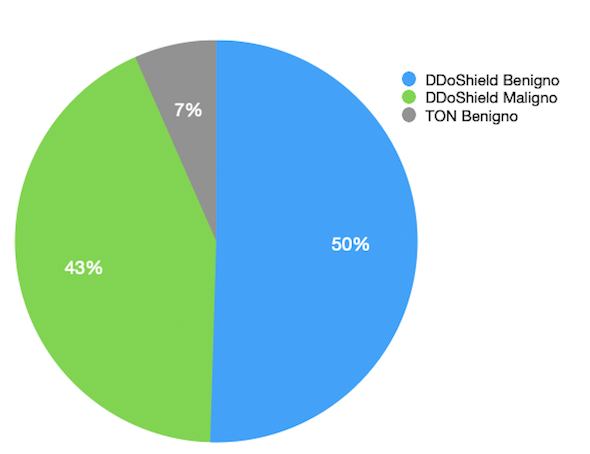
\includegraphics[scale= 0.8]{UNINA_MSc_Thesis_Project/img/chapterRisulati/composizione_DATASET_1 centrata.png}
  \caption{Composizione Dataset 1}
\end{figure}

\begin{table}[htbp]
\centering
\renewcommand{\arraystretch}{1.5} % Aumenta lo spazio tra le righe
\resizebox{\textwidth}{!}{ % Ridimensiona la tabella alla larghezza del testo
\begin{tabular}{|p{4cm}|p{3cm}|p{3cm}|p{3cm}|p{3cm}|}
\hline
\textbf{Modello} & \textbf{Accuracy \%} & \textbf{Precision \%} & \textbf{Recall \%} & \textbf{F1-Score \%} \\
\hline
\textbf{K-Means} & 84.09 & 76.54 & 98.95 & 86.31 \\
\hline
\textbf{Random Forest (RF-0.25)} & 70.74 & 100 & 42.17 & 59.32 \\
\hline
\textbf{Convolutional Neural Network (CNN)} & 66.34 & 99.66 & 33.42 & 50.06 \\
\hline
\end{tabular}
}
\caption{Metriche di performance per Dataset 1}
\label{tab:performance_metrics}
\end{table}

Il \textbf{Dataset 1} contiene traffico benigno e maligno proveniente da DDoShield, insieme al traffico benigno dal dataset TON\_IOT. I risultati ottenuti per questo dataset evidenziano una performance discreta da parte del modello \textit{K-Means}, che ha raggiunto un'accuratezza di 0.84, una precisione di 0.76, un richiamo elevato pari a 0.98 e un F1-Score di 0.86. Questo suggerisce che il modello ha una forte capacità di rilevare traffico maligno (alto richiamo), ma tende a classificare una parte del traffico benigno come maligno (Falsi Positivi), riflettendo la precisione relativamente bassa.
 
Al contrario, il \textit{CNN} ha ottenuto risultati inferiori rispetto al \textit{K-Means}, con un'accuratezza di 0.66 e un F1-Score di 0.50, indicando che il modello soffre di una bassa capacità di rilevamento del traffico maligno (richiamo di 0.33), pur mantenendo una precisione molto alta (0.99), evidenziando una tendenza a minimizzare i falsi positivi.
L'algoritmo \textit{RF} presenta prestazioni accettabili solo scegliendo una soglia minore di 0.5.
Ulteriori aspetti saranno approfonditi in seguito nel paragrafo conclusivo.

\subsection{Dataset 2}

\begin{figure}[htbp]
\centering
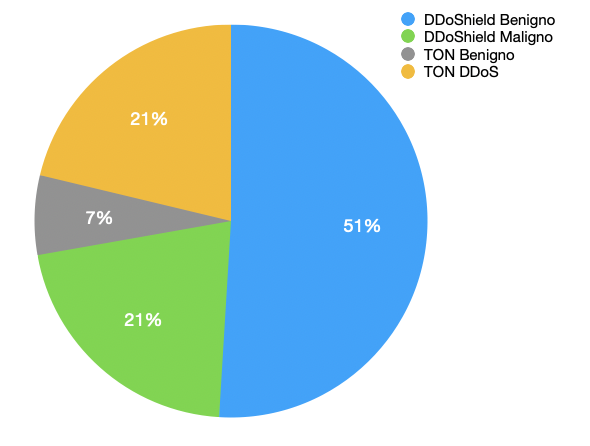
\includegraphics[scale= 0.8]{UNINA_MSc_Thesis_Project/img/chapterRisulati/composizione_DATASET_2.png}
  \caption{Composizione Dataset 2}
\end{figure}


\begin{table}[htbp]
\centering
\renewcommand{\arraystretch}{1.5} % Aumenta lo spazio tra le righe
\resizebox{\textwidth}{!}{ % Ridimensiona la tabella alla larghezza del testo
\begin{tabular}{|p{4cm}|p{3cm}|p{3cm}|p{3cm}|p{3cm}|}
\hline
\textbf{Modello} & \textbf{Accuracy \%} & \textbf{Precision \%} & \textbf{Recall \%} & \textbf{F1-Score \%} \\
\hline
\textbf{K-Means} & 86.53 & 79.60 & 98.75 & 88.14 \\
\hline
\textbf{Random Forest (RF-0.25)} & 97.40  & 95.11 & 100 & 97.49  \\
\hline
\textbf{Random Forest (RF)} & 99.95 & 99.90 & 100 & 99.95 \\
\hline
\textbf{Convolutional Neural Network (CNN)} & 99.98 & 100 & 99.97 & 99.98 \\
\hline
\end{tabular}
}
\caption{Metriche di performance per Dataset 2}
\label{tab:performance_metrics}
\end{table}

Il \textbf{Dataset 2} è stato generato combinando il traffico benigno di \textit{Dataset 1} con traffico maligno equamente distribuito tra DDoShield e TON\_IOT DDoS. Qui, \textit{K-Means} ha ottenuto risultati superiori rispetto al \textit{Dataset 1}, con un'accuratezza di 0.86 e un F1-Score di 0.88. Il miglioramento delle prestazioni si riflette anche in una precisione maggiore (0.79), che indica una riduzione dei falsi positivi.
\textit{Random Forest} ha mostrato eccellenti performance, con valori quasi perfetti (accuracy di 0.99, F1-Score di 0.99), dimostrando una notevole capacità di bilanciare la rilevazione degli attacchi tra DDoShield e TON\_IOT.
La \textit{CNN} ha ottenuto risultati simili a quelli di \textit{Random Forest}, con un'accuratezza di 0.99, mostrando come i modelli più complessi possano gestire efficacemente dataset bilanciati.

\subsection{Dataset 3}

\begin{figure}[htbp]
\centering
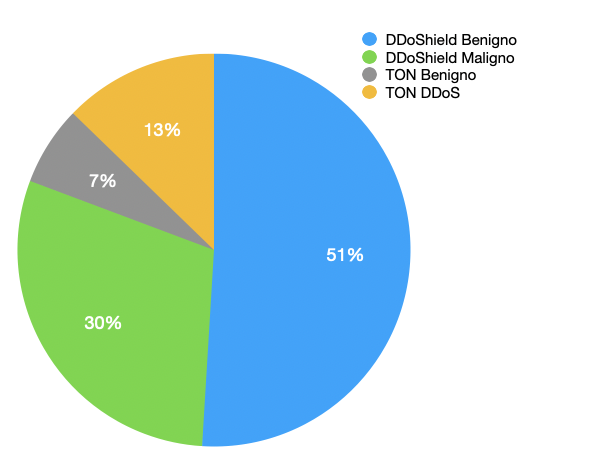
\includegraphics[scale= 0.8]{UNINA_MSc_Thesis_Project/img/chapterRisulati/composizione_DATASET_3.png}
  \caption{Composizione Dataset 3}
\end{figure}

\begin{table}[htbp]
\centering
\renewcommand{\arraystretch}{1.5} % Aumenta lo spazio tra le righe
\resizebox{\textwidth}{!}{ % Ridimensiona la tabella alla larghezza del testo
\begin{tabular}{|p{4cm}|p{3cm}|p{3cm}|p{3cm}|p{3cm}|}
\hline
\textbf{Modello} & \textbf{Accuracy \%} & \textbf{Precision \%} & \textbf{Recall \%} & \textbf{F1-Score \%} \\
\hline
\textbf{K-Means} & 86.62  & 80.71 & 96.74 & 88.00 \\
\hline
\textbf{Random Forest (RF-0.25)} & 91.18 & 1.0 & 42.17 & 95.38 \\
\hline
\textbf{Random Forest (RF)} & 100 & 100 & 100 & 100 \\
\hline
\textbf{Convolutional Neural Network (CNN)} & 67.90 & 100 & 36.41 & 53.38 \\
\hline
\end{tabular}
}
\caption{Metriche di performance per Dataset 3}
\label{tab:performance_metrics}
\end{table}

Nel \textbf{Dataset 3}, con una prevalenza di traffico maligno da DDoShield, \textit{K-Means} ha ottenuto prestazioni comparabili al \textit{Dataset 2}, con un'accuratezza di 0.86 e un F1-Score di 0.88, mantenendo un buon bilanciamento tra precisione e richiamo.
\textit{Random Forest} ha nuovamente raggiunto risultati perfetti, dimostrando la sua capacità di gestire dataset sbilanciati. Tuttavia, la \textit{CNN} ha sofferto un calo significativo (accuratezza di 0.67 e F1-Score di 0.53), indicando che l'architettura neurale potrebbe avere difficoltà nel rilevare intrusioni in dataset con distribuzioni sbilanciate tra diverse tipologie di traffico maligno.

\subsection{Dataset 4}

\begin{figure}[htbp]
\centering
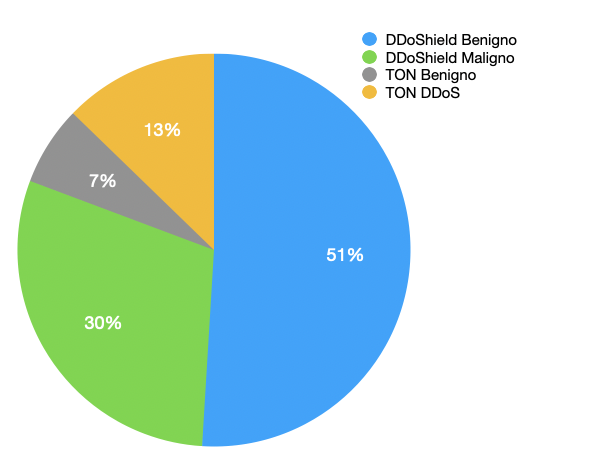
\includegraphics[scale= 0.8]{UNINA_MSc_Thesis_Project/img/chapterRisulati/composizione_DATASET_4.png}
  \caption{Composizione Dataset 4}
\end{figure}

\begin{table}[htbp]
\centering
\renewcommand{\arraystretch}{1.5} % Aumenta lo spazio tra le righe
\resizebox{\textwidth}{!}{ % Ridimensiona la tabella alla larghezza del testo
\begin{tabular}{|p{4cm}|p{3cm}|p{3cm}|p{3cm}|p{3cm}|}
\hline
\textbf{Modello} & \textbf{Accuracy \%} & \textbf{Precision \%} & \textbf{Recall \%} & \textbf{F1-Score \%} \\
\hline
\textbf{K-Means} & 84.07  & 78.26 & 94.97 & 85.81 \\
\hline
\textbf{Random Forest (RF-0.25)} & 93.30 & 88.28 & 100 & 93.78 \\
\hline
\textbf{Random Forest (RF)} & 99.91 & 99.83 & 100 & 99.91 \\
\hline
\textbf{Convolutional Neural Network (CNN)} & 99.60 & 100 & 99.22 & 99.60 \\
\hline
\end{tabular}
}
\caption{Metriche di performance per Dataset 4}
\label{tab:performance_metrics}
\end{table}

Nel \textbf{Dataset 4}, caratterizzato da una maggioranza di traffico maligno da TON\_IOT DDoS, \textit{K-Means} ha mostrato una leggera diminuzione delle performance (accuratezza di 0.84, F1-Score di 0.85), a causa di un aumento dei falsi positivi, come indicato dalla precisione di 0.78.
\textit{Random Forest} continua a mantenere prestazioni eccellenti, con un'accuratezza di 0.9991 e metriche molto elevate, mentre la \textit{CNN}, con un'accuratezza di 0.99, ha dimostrato di gestire meglio dataset con una predominanza di traffico maligno da TON\_IOT rispetto a quanto visto nel \textit{Dataset 3}.

\subsection{Dataset 5}

\begin{figure}[htbp]
\centering
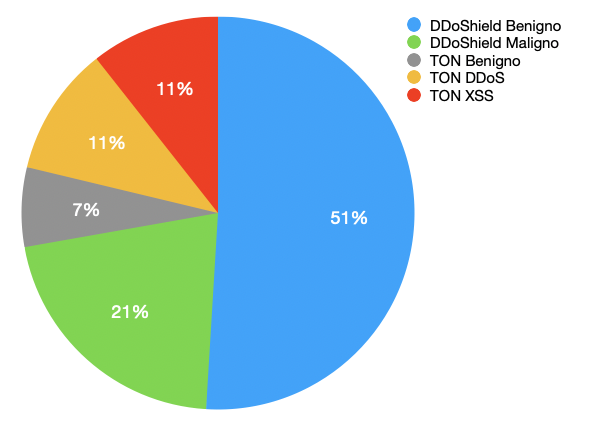
\includegraphics[scale= 0.8]{UNINA_MSc_Thesis_Project/img/chapterRisulati/composizione_DATASET_5.png}
  \caption{Composizione Dataset 5}
\end{figure}

\begin{table}[htbp]
\centering
\renewcommand{\arraystretch}{1.5} % Aumenta lo spazio tra le righe
\resizebox{\textwidth}{!}{ % Ridimensiona la tabella alla larghezza del testo
\begin{tabular}{|p{4cm}|p{3cm}|p{3cm}|p{3cm}|p{3cm}|}
\hline
\textbf{Modello} & \textbf{Accuracy \%} & \textbf{Precision \%} & \textbf{Recall \%} & \textbf{F1-Score \%} \\
\hline
\textbf{K-Means} & 86.31  & 86.42 & 94.48 & 90.27 \\
\hline
\textbf{Random Forest (RF-0.25)} & 76.48 & 74.04 & 100 & 85.08 \\
\hline
\textbf{Random Forest (RF)} & 99.99 & 99.99 & 100 & 99.99 \\
\hline
\textbf{Convolutional Neural Network (CNN)} & 96.96 & 99.96 & 95.50 & 97.68 \\
\hline
\end{tabular}
}
\caption{Metriche di performance per Dataset 5}
\label{tab:performance_metrics}
\end{table}

Il \textbf{Dataset 5} introduce traffico XSS nel dataset, rendendo la classificazione più complessa. Nonostante ciò, \textit{K-Means} ha mantenuto buone prestazioni con un'accuratezza di 0.8631 e un F1-Score di 0.90. La precisione è aumentata (0.86), suggerendo che il modello ha migliorato la sua capacità di evitare falsi positivi in presenza di una maggiore varietà di traffico maligno.

\textit{Random Forest} ha nuovamente raggiunto valori quasi perfetti (accuratezza di 0.99), dimostrando la sua capacità di rilevare diverse tipologie di attacchi con alta precisione. La \textit{CNN} ha mostrato una buona capacità di generalizzazione, con un'accuratezza di 0.96 e un F1-Score di 0.97, dimostrando che riesce a gestire anche dataset più complessi con traffico misto (DDoS e XSS).

\subsection{Analisi dei Risultati}
In questa sezione analizziamo i risultati ottenuti dai vari algoritmi applicati sui differenti dataset descritti in precedenza. Ogni algoritmo ha mostrato prestazioni diverse a seconda delle caratteristiche del dataset, il che ci permette di identificare alcune peculiarità nei loro comportamenti.

\subsubsection{K-Means}
\textit{K-Means} è un algoritmo di clustering non supervisionato che raggruppa i dati basandosi sulla similarità, utilizzando la distanza euclidea per creare cluster. Sebbene non sia nato come algoritmo di classificazione, può essere adattato per tale scopo. Tuttavia, ha dimostrato prestazioni variabili a seconda del dataset considerato.
Nel \textbf{Dataset 1} e nel \textbf{Dataset 2}, dove la separazione tra classi è relativamente chiara, \textit{K-Means} ha ottenuto ottimi risultati, con accuratezze superiori all'84\%. Questo suggerisce che l'algoritmo riesce a sfruttare efficacemente la differenza strutturale tra traffico benigno e maligno quando questa è ben definita.
Con dataset più complessi, come il \textbf{Dataset 3} e il \textbf{Dataset 4}, in cui c'è uno squilibrio tra le classi, \textit{K-Means} ha mostrato un leggero calo delle performance. Sebbene la precisione sia rimasta alta (indicando che il modello fa poche previsioni errate quando etichetta un pacchetto come maligno), l'accuratezza complessiva e il richiamo sono diminuiti leggermente. Questo è indicativo del fatto che \textit{K-Means} fatica a distinguere intrusioni meno evidenti, suggerendo che l'algoritmo è eccessivamente conservativo nel segnalare traffico maligno, risultando in un elevato numero di falsi negativi.

\subsubsection{Random Forest (RF)}
\textit{Random Forest} è un algoritmo di classificazione supervisato che utilizza un insieme di alberi decisionali per creare un modello robusto. Grazie alla sua capacità di catturare interazioni complesse tra le variabili, RF ha ottenuto eccellenti prestazioni su quasi tutti i dataset, mantenendo accuratezze vicine al 100\%.
In particolare, \textit{Random Forest} ha gestito in modo eccellente i dataset più complessi come il \textbf{Dataset 3} e il \textbf{Dataset 5}, dove il traffico maligno proveniva da fonti diverse (DDoS e XSS) e presentava una variabilità maggiore. Le alte prestazioni di RF sono dovute alla capacità dell'algoritmo di gestire la variabilità dei dati e catturare pattern non lineari, riducendo così il rischio di falsi negativi o positivi. Questo conferma l'idoneità di \textit{Random Forest} nel contesto della rilevazione delle intrusioni, anche in scenari con distribuzioni di dati complesse e sbilanciate.

\subsubsection{Convolutional Neural Network (CNN)}
Le \textit{Convolutional Neural Networks} sono reti neurali particolarmente adatte all'analisi di dati con struttura gerarchica, come immagini o dati con pattern temporali. Tuttavia, le prestazioni della \textit{CNN} sono state variabili a seconda del dataset utilizzato.
Nel \textbf{Dataset 1} e \textbf{Dataset 3}, la CNN ha mostrato prestazioni inferiori rispetto agli altri algoritmi, con un'accuratezza di circa il 66\% e il 68\%, rispettivamente. Questo può essere attribuito al fatto che questi dataset non fornivano sufficiente complessità o variazione nei dati per permettere alla CNN di esprimere appieno le sue capacità. In particolare, nel \textbf{Dataset 3}, la precisione è risultata molto alta (1.0), ma il richiamo è stato estremamente basso (0.36), indicando che la CNN era estremamente selettiva nel classificare un pacchetto come maligno, trascurando però molti pacchetti malevoli (alto numero di falsi negativi).
D'altro canto, nel \textbf{Dataset 5}, che conteneva traffico DDoS e XSS, la CNN ha mostrato le sue migliori prestazioni, con un'accuratezza del 96.96\%. In questo caso, la complessità dei dati ha permesso alla CNN di identificare più efficacemente pattern distintivi tra le diverse tipologie di attacchi.

\subsubsection{Sintesi dell'analisi}
L'analisi dei risultati mostra che le differenze nelle prestazioni degli algoritmi dipendono principalmente dalla complessità del dataset e dalla distribuzione delle classi:
\begin{itemize}
\item \textbf{K-Means} funziona bene su dataset bilanciati e con classi chiaramente separate, come \textit{Dataset 1} e \textit{Dataset 2}. Tuttavia, fatica in presenza di classi meno ben distinte o dataset più complessi con un numero di falsi positivi che potrebbe aumentare.
\item \textbf{Random Forest} si dimostra un algoritmo flessibile e robusto, con prestazioni costantemente elevate su tutti i dataset, grazie alla sua capacità di gestire interazioni complesse e dati sbilanciati.
\item \textbf{CNN} mostra prestazioni variabili, eccellendo solo nei dataset più complessi (\textit{Dataset 5}), dove è in grado di identificare pattern intricati. Tuttavia, ha evidenziato difficoltà con dataset fortemente sbilanciati come il \textit{Dataset 3} e con pochi dati a supporto, suggerendo che potrebbe necessitare di ulteriori ottimizzazioni per gestire questi scenari.
\end{itemize}
In particolare, è importante sottolineare che \textit{Random Forest} è un algoritmo capace di cogliere relazioni non lineari, il che si riflette in un comportamento più bilanciato anche in presenza di dataset eterogenei. Le reti neurali, sebbene siano in grado di rilevare pattern complessi cosi come \textit{Random Forest}, soffrono maggiormente \textbf{la dipendenza dai dati} e richiedono una mole maggiore di dati per un addestramento efficace. Questo spiega i risultati inferiori ottenuti sui \textit{Dataset 1} e \textit{Dataset 3}, che sono fortemente sbilanciati a favore del simulatore.
Concludendo, \textbf{Random Forest} emerge come la scelta più solida per la rilevazione delle intrusioni nei dataset utilizzati, mentre \textit{CNN} e \textit{K-Means} mostrano prestazioni buone solo in contesti specifici, a seconda della struttura dei dati.

\section{L'impatto della strategia}

Per valutare l'impatto della tecnica di addestramento e del lavoro svolto, in questa sezione analizziamo gli stessi dataset senza l'uso del simulatore \textit{DDoShield}. L'obiettivo è simulare scenari nei quali non avremmo avuto il supporto del simulatore, consentendo di valutare il contributo effettivo di \textit{DDoShield} in condizioni reali. Il confronto delle performance con e senza il simulatore è fondamentale per dimostrare l'importanza del tool, soprattutto in presenza di dataset fortemente sbilanciati. In questi casi, infatti, vedremo come i dati, senza il simulatore, risulterebbero difficilmente utilizzabili.

Le metriche nelle tabelle seguenti saranno presentate nel seguente formato:
\[metrica\_DATASET\_TON\_Only_i [metrica\_DATASET_i]\]
dove \[DATASET_i\] con i=1,2,3,4,5 rappresenta gli scenari precedentemente generati.



\subsection{Dataset2 TON\_Only}

\begin{figure}[htbp]
\centering
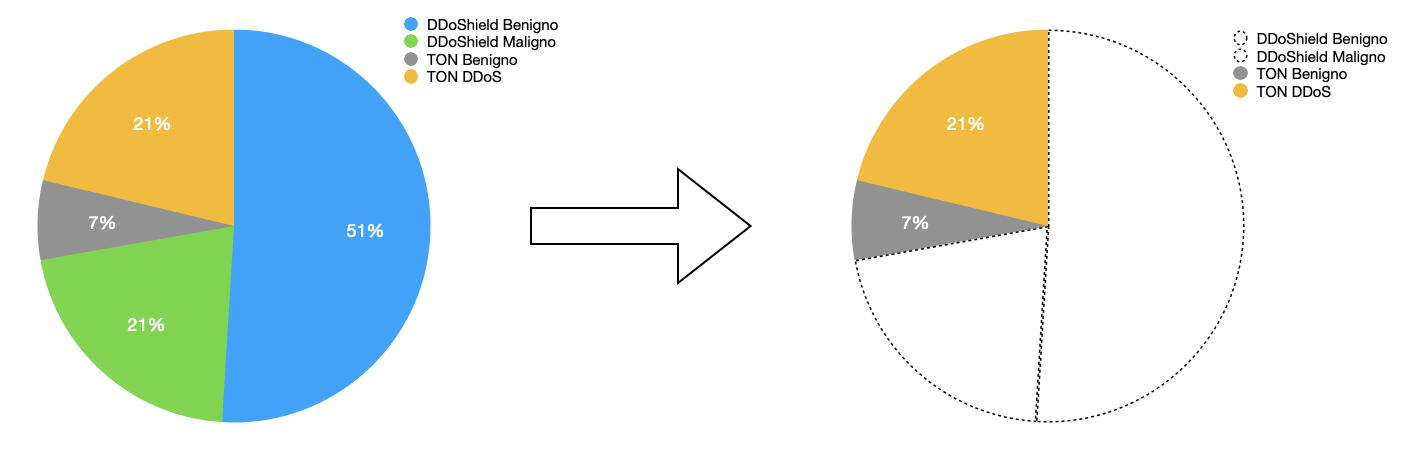
\includegraphics[scale= 0.6]{UNINA_MSc_Thesis_Project/img/chapterRisulati/TON_Only/composizione_TON_ONLY2.png}
  \caption{Composizione Dataset TON Only 2}
\end{figure}

\begin{table}[htbp]
\centering
\renewcommand{\arraystretch}{1.5}
\resizebox{\textwidth}{!}{
\begin{tabular}{|p{4cm}|p{3cm}|p{3cm}|p{3cm}|p{3cm}|}
\hline
\textbf{Modello} & \textbf{Accuracy \%} & \textbf{Precision \%} & \textbf{Recall \%} & \textbf{F1-Score \%} \\
\hline
\textbf{K-Means} & 98.47 [86.53] & 97.49 [79.60] & 99.57 [98.75] & 98.52 [88.14] \\
\hline
\textbf{Random Forest (RF-0.25)} & 49.34 [97.40] & 100 [95.11] & 0.02 [100] & 0.05 [97.49] \\
\hline
\textbf{Random Forest (RF-0.5)} & 49.34 [99.95] & 0 [99.90] & 0 [100] & 0 [99.95] \\
\hline
\textbf{Convolutional Neural Network (CNN)} & 93.16 [99.98] & 99.68 [100] & 86.77 [99.97] & 92.78 [99.98] \\
\hline
\end{tabular}
}
\caption{Metriche di performance per Dataset2 TON\_Only}
\label{tab:performance_metrics}
\end{table}
Nel Dataset2, l'uso del simulatore ha un impatto positivo su tutti i modelli, tranne che su \textit{K-Means}, dove la differenza è meno pronunciata. In particolare, il \textit{Random Forest} senza simulatore mostra risultati estremamente scarsi, con un \textit{recall} praticamente nullo, mentre con il simulatore il modello raggiunge performance ottimali in tutte le metriche. La \textit{CNN} mostra un comportamento simile, con un significativo miglioramento nell'accuratezza, precisione e \textit{recall} grazie al simulatore.

\subsection{Dataset3 TON\_Only}

\begin{figure}[htbp]
\centering
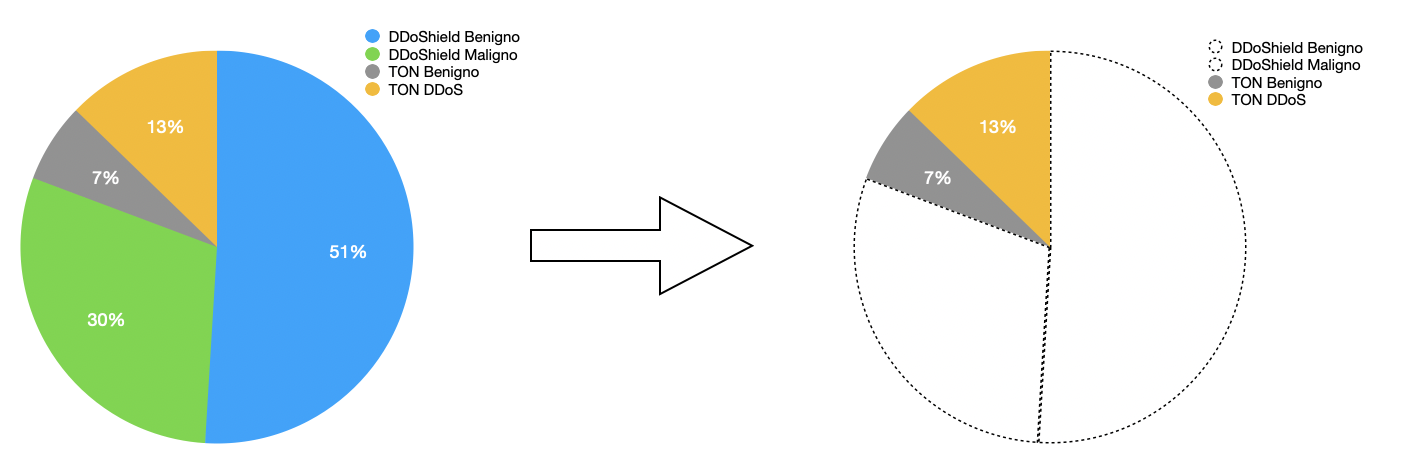
\includegraphics[scale= 0.6]{UNINA_MSc_Thesis_Project/img/chapterRisulati/TON_Only/composizione_TON_ONLY3.png}
  \caption{Composizione Dataset TON Only 3}
\end{figure}


\begin{table}[htbp]
\centering
\renewcommand{\arraystretch}{1.5}
\resizebox{\textwidth}{!}{
\begin{tabular}{|p{4cm}|p{3cm}|p{3cm}|p{3cm}|p{3cm}|}
\hline
\textbf{Modello} & \textbf{Accuracy \%} & \textbf{Precision \%} & \textbf{Recall \%} & \textbf{F1-Score \%} \\
\hline
\textbf{K-Means} & 97.40 [86.62] & 95.15 [80.71] & 100 [96.74] & 97.51 [88.00] \\
\hline
\textbf{Random Forest (RF-0.25)} & 57.72 [95.11] & 54.51 [91.18] & 100 [100] & 70.56 [95.38] \\
\hline
\textbf{Random Forest (RF-0.5)} & 86.44 [100] & 78.12 [100] & 100 [100] & 88.29 [100] \\
\hline
\textbf{Convolutional Neural Network (CNN)} & 98.89 [67.90] & 97.87 [100] & 100 [36.41] & 98.92 [53.38] \\
\hline
\end{tabular}
}
\caption{Metriche di performance per Dataset3 TON\_Only}
\label{tab:performance_metrics}
\end{table}
Nel Dataset3, il simulatore migliora significativamente le prestazioni del \textit{Random Forest}. Nel \textit{K-Means}, i risultati senza simulatore sono più elevati. La \textit{CNN} mostra un comportamento interessante: mentre la precisione rimane alta, il \textit{recall} e quindi anche l'F1-score peggiorano drasticamente senza simulatore, ricordiamo che questo dataset risultava pesantemente sbilanciato ai dati del simulatore. 

\subsection{Dataset4 TON\_Only}

\begin{figure}[htbp]
\centering
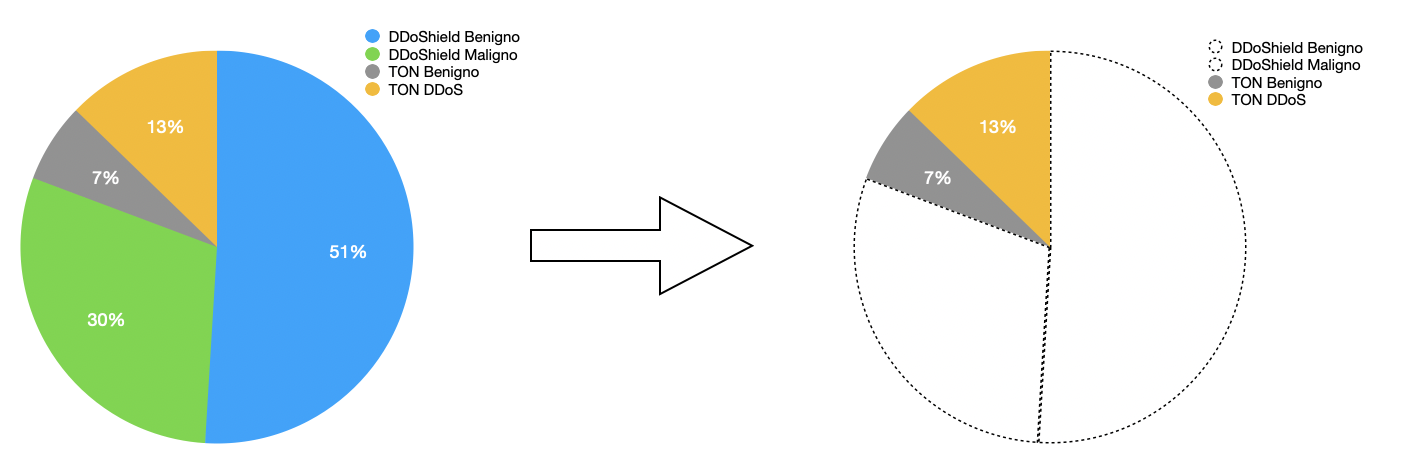
\includegraphics[scale= 0.6]{UNINA_MSc_Thesis_Project/img/chapterRisulati/TON_Only/composizione_TON_ONLY4.png}
  \caption{Composizione Dataset TON Only 4}
\end{figure}

\begin{table}[htbp]
\centering
\renewcommand{\arraystretch}{1.5}
\resizebox{\textwidth}{!}{
\begin{tabular}{|p{4cm}|p{3cm}|p{3cm}|p{3cm}|p{3cm}|}
\hline
\textbf{Modello} & \textbf{Accuracy \%} & \textbf{Precision \%} & \textbf{Recall \%} & \textbf{F1-Score \%} \\
\hline
\textbf{K-Means} & 97.03 [84.07] & 94.50 [78.26] & 100 [94.97] & 97.17 [85.81] \\
\hline
\textbf{Random Forest (RF-0.25)} & 57.18 [93.30] & 54.14 [88.28] & 100 [100] & 70.00 [93.78] \\
\hline
\textbf{Random Forest (RF-0.5)} & 86.21 [99.91] & 78.46 [99.83] & 100 [100] & 88.46 [99.91] \\
\hline
\textbf{Convolutional Neural Network (CNN)} & 98.82 [99.60] & 97.72 [100] & 100 [99.22] & 98.85 [99.60] \\
\hline
\end{tabular}
}
\caption{Metriche di performance per Dataset4 TON\_Only}
\label{tab:performance_metrics}
\end{table}

Per il Dataset4, si osserva un miglioramento generale delle performance con l'uso del simulatore, specialmente per \textit{Random Forest} e \textit{CNN}, mentre il \textit{K-Means} risulta più stabile anche senza simulatore. Questo indica che il simulatore aiuta i modelli più complessi a gestire meglio dataset con distribuzioni più eterogenee e difficili da prevedere.

\subsection{Dataset5 TON\_Only}

\begin{figure}[htbp]
\centering
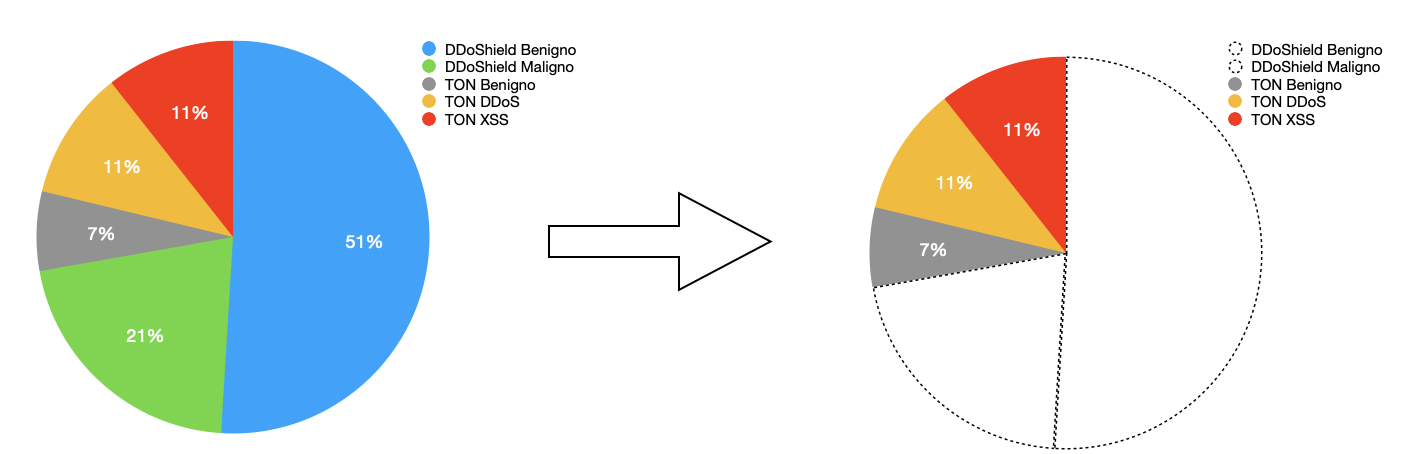
\includegraphics[scale= 0.6]{UNINA_MSc_Thesis_Project/img/chapterRisulati/TON_Only/composizione_TON_ONLY5.png}
  \caption{Composizione Dataset TON Only 5}
\end{figure}

\begin{table}[htbp]
\centering
\renewcommand{\arraystretch}{1.5}
\resizebox{\textwidth}{!}{
\begin{tabular}{|p{4cm}|p{3cm}|p{3cm}|p{3cm}|p{3cm}|}
\hline
\textbf{Modello} & \textbf{Accuracy \%} & \textbf{Precision \%} & \textbf{Recall \%} & \textbf{F1-Score \%} \\
\hline
\textbf{K-Means} & 97.85 [86.31] & 96.03 [86.42] & 99.92 [94.48] & 97.94 [90.27] \\
\hline
\textbf{Random Forest (RF-0.25)} & 52.28 [76.48] & 51.50 [74.04] & 100 [100] & 67.99 [85.08] \\
\hline
\textbf{Random Forest (RF-0.5)} & 99.90 [99.99] & 99.92 [99.99] & 100 [100] & 99.91 [99.99] \\
\hline
\textbf{Convolutional Neural Network (CNN)} & 98.50 [96.96] & 98.25 [99.96] & 99.85 [95.50]
 & 98.92 [97.68] \\
\hline
\end{tabular}
}
\caption{Metriche di performance per Dataset5 TON\_Only}
\label{tab:performance_metrics}
\end{table}

Anche nel Dataset5, l'uso del simulatore porta a miglioramenti significativi per tutti i modelli, ad eccezione del \textit{K-Means} che mostra performance più elevate senza il simulatore. Questo comportamento potrebbe essere dovuto alla capacità del \textit{K-Means} di lavorare meglio con i dati "naturali" e meno strutturati.

\subsection{Conclusioni Generali sui Risultati}

Dai risultati ottenuti attraverso i vari dataset, possiamo trarre diverse conclusioni riguardo l'efficacia del simulatore \textit{DDoShield} e il suo impatto sulle prestazioni dei modelli testati.
In generale, l'utilizzo del simulatore ha migliorato significativamente le prestazioni di modelli complessi come \textit{Random Forest} e \textit{Convolutional Neural Network (CNN)}. Questo miglioramento è particolarmente evidente in dataset sbilanciati, dove il simulatore ha fornito un contributo fondamentale per bilanciare le classi e consentire al modello di apprendere meglio anche in presenza di attacchi più rari o complessi. Le metriche di \textit{accuracy}, \textit{precision}, \textit{recall} e \textit{F1-score} mostrano chiaramente che, senza il simulatore, i modelli soffrono di un significativo calo di performance, specialmente in termini di \textit{recall} e \textit{F1-score}, suggerendo difficoltà nel riconoscere correttamente le classi di attacco.
D'altra parte, il modello \textit{K-Means} ha mostrato un comportamento meno dipendente dal simulatore, con risultati sempre migliori senza l'uso di dati simulati.

\textbf{Random Forest}: Il \textit{Random Forest} ha tratto il massimo beneficio dal simulatore, passando da performance pessime in assenza del simulatore a performance ottimali quando i dati simulati erano inclusi. Ciò indica che il modello è altamente sensibile al bilanciamento delle classi e alla varietà dei dati, che il simulatore è stato in grado di fornire. Senza il simulatore, infatti, in alcuni casi il modello non riusciva nemmeno a identificare correttamente le classi di attacco, con un \textit{recall} e un \textit{F1-score} prossimi allo zero.

\textbf{Convolutional Neural Network (CNN)}: Anche il modello \textit{CNN} ha beneficiato significativamente dell'uso del simulatore, mostrando un miglioramento in quasi tutte le metriche. Tuttavia, sono emersi anche casi in cui il modello ha presentato un calo di performance nel \textit{recall}, specialmente per dataset molto sbilanciati. Questo suggerisce che, sebbene il simulatore abbia migliorato la capacità della \textit{CNN} di apprendere dai dati, rimane una certa vulnerabilità del modello nel gestire alcune classi di attacco più complesse e povere di dati.

\textbf{K-Means}: L'algoritmo \textit{K-Means} presenta un caso particolare, poiché per tutti i dataset testati le performance sono risultate superiori senza l'uso dei dati simulati. Questo suggerisce che i cluster naturali nel dataset non simulato sono più facilmente identificabili da algoritmi di clustering non supervisionato rispetto ai dati generati. Questa condizione porta a performance molto elevate anche in presenza di un numero ridotto di dati, come nel \textit{Dataset 4}. In questo caso, l'introduzione del simulatore genera un aumento del rumore, comportando una difficoltà nelle predizioni.

\subsection{Conclusioni}
Complessivamente, i risultati indicano che il simulatore \textit{DDoShield} ha un impatto estremamente positivo sui modelli di apprendimento supervisionato, come \textit{Random Forest} e \textit{CNN}, migliorando significativamente la capacità di questi modelli di gestire dataset sbilanciati e di riconoscere correttamente le classi di attacco. Inoltre, il simulatore risulta comunque utile anche con \textit{K-Means}, per evitare problemi di overfitting.
Pertanto, possiamo concludere che l'uso di un simulatore come \textit{DDoShield} è fortemente raccomandato in scenari di classificazione e riconoscimento di attacchi, in particolare quando si impiegano modelli di apprendimento supervisionato e si lavora con dataset sbilanciati. 

%Tuttavia, nel caso di algoritmi come le CNN, è fondamentale prestare attenzione a non introdurre una quantità eccessiva di dati simulati, poiché ciò potrebbe ri-sbilanciare il dataset. Gli esperimenti condotti suggeriscono di mantenere la proporzione di dati simulati al di sotto del 70\% per garantire risultati ottimali.


\section{Repository GitHub}

Tutto il codice sviluppato e i dataset utilizzati per questa tesi sono disponibili pubblicamente su GitHub. Questa repository è stato creata con l'obiettivo di garantire la riproducibilità del lavoro svolto, consentendo ad altri ricercatori e professionisti di replicare gli esperimenti e, eventualmente, migliorare le metodologie proposte. 

La repository GitHub include i seguenti elementi:
\begin{itemize}
    \item Il codice sorgente per la generazione dei dataset utilizzati nei diversi esperimenti.
    \item Gli script utilizzati per l'addestramento dei modelli di machine learning, inclusi ulteriori algoritmi oltre quelli proposti in questo lavoro.
    %\item I risultati ottenuti, presentati in forma di report e grafici che riassumono le metriche di valutazione per ogni modello.
    \item La documentazione tecnica relativa al setup dell'ambiente di simulazione e alla creazione dei dataset a partire dai pacchetti catturati durante il traffico di rete.
\end{itemize}
Per accedere alla repository, è possibile visitare il seguente link:

\begin{quote}
\href{https://github.com/Luigi-Cerrato/ThesisRepository}{https://github.com/Luigi-Cerrato/ThesisRepository}
\end{quote}
La pubblicazione su GitHub non solo rende i dati e il codice liberamente accessibili, ma promuove anche un approccio collaborativo e aperto alla ricerca. Chiunque può contribuire con suggerimenti, correzioni o ulteriori sviluppi attraverso il sistema di pull request e issue tracking messo a disposizione dalla piattaforma.
In un contesto di ricerca sempre più orientato verso l'open science, questa scelta riflette l'importanza di condividere conoscenze e strumenti per accelerare i progressi nel campo della sicurezza informatica e dell'addestramento di Intrusion Detection Systems (IDS).

\chapter{Conclusioni e Sviluppi futuri}
In conclusione, il lavoro svolto in questa tesi rappresenta un punto di partenza solido per l'ottimizzazione dei sistemi di rilevamento degli attacchi basati su dati simulati. Tuttavia, esistono molteplici direzioni per futuri sviluppi. La costante evoluzione del panorama delle minacce e delle tecnologie richiede un continuo aggiornamento delle tecniche e degli strumenti impiegati, e la ricerca futura potrà trarre grande vantaggio dall'integrazione di nuove tecnologie di simulazione, machine learning e data augmentation.
L'impatto della data augmentation è stato significativo, mostrando come alcuni dataset inizialmente inutilizzabili in condizioni reali potessero migliorare notevolmente grazie all'inserimento di un tool come il simulatore \textit{DDoShield}. Questa metodologia consente, in particolar modo, di affrontare situazioni in cui è difficile raccogliere dati reali sufficienti, come ad esempio nei casi in cui il sistema è nuovo o non ha ancora affrontato un numero consistente di minacce. La possibilità di simulare scenari permette di ampliare la base dati, rendendo il sistema più robusto e preparato ad affrontare scenari complessi di attacco.
Tuttavia, ci sono diversi spunti di miglioramento che potrebbero essere esplorati in studi futuri. Di seguito valutiamo alcune possibilità.

\section{Ottimizzazione delle tecniche di simulazione}
Sebbene il simulatore abbia dimostrato un grande potenziale, rimane spazio per migliorare la qualità e l'affidabilità dei dati simulati. Futuri sviluppi potrebbero concentrarsi sull'ottimizzazione del processo di simulazione, introducendo tecniche di simulazione più avanzate che generino dati ancor più realistici e che si adattino meglio alle peculiarità dei singoli scenari di attacco. Ad esempio, potrebbe essere utile esplorare l'integrazione di metodi di machine learning ed algoritmi genetici nella generazione dei dati simulati(specie se si usano protocolli), per creare scenari di attacco più dinamici e realistici. 
Potrebbero inoltre essere introdotti nuovi attacchi ricostruendo cosi nuovi scenari sempre più complessi.

\section{Integrazione con altre tecniche di Data Augmentation}
Lo sviluppo futuro potrebbe anche includere l'integrazione con altre tecniche di \textit{data augmentation}, come il \textit{data synthesis} o il \textit{GAN-based augmentation} (Generative Adversarial Networks), che potrebbero ulteriormente aumentare la varietà dei dati disponibili.\cite{GAN} Questo approccio combinato potrebbe permettere di creare dataset ancora più ricchi e diversificati, migliorando la capacità dei modelli di apprendimento di riconoscere un ampio spettro di attacchi, anche quelli meno frequenti o inediti.

\section{Valutazione dell'impatto su altri algoritmi di Machine Learning}
Un altro ambito di sviluppo futuro è l'estensione dell'analisi a ulteriori algoritmi di machine learning oltre a quelli già utilizzati (K-Means, Random Forest, CNN). Sarebbe interessante valutare l'impatto del simulatore e delle tecniche di \textit{data augmentation} su modelli più recenti, come le reti neurali ricorrenti (RNN) che potrebbero offrire performance migliori, soprattutto in scenari di attacchi altamente dinamici o con caratteristiche temporali complesse. \cite{RNN}

\section{Monitoraggio e aggiornamento continuo del simulatore}
In un contesto di sicurezza informatica, le minacce evolvono costantemente. Pertanto, sarebbe auspicabile sviluppare un sistema di monitoraggio continuo e di aggiornamento del simulatore in modo da adattarlo ai nuovi tipi di attacchi. Questo processo dinamico permetterebbe al simulatore di restare sempre aggiornato, migliorando così le capacità di previsione e reazione del sistema. L'integrazione di un framework di apprendimento continuo (\textit{online learning}) potrebbe rappresentare un'opportunità interessante per questo tipo di evoluzione.

\section{Collaborazione tra più simulazioni e framework}
Un altro aspetto interessante da considerare sarebbe la collaborazione tra simulatori differenti o l'integrazione di più framework all'interno della stessa pipeline di addestramento. Unendo simulazioni diverse, provenienti da tool come \textit{DDoShield}, con altre fonti di dati (come honeypots, reti reali attaccate e attività di penetration testing), si potrebbe ulteriormente migliorare la qualità e la copertura del dataset, ampliando le capacità di difesa del sistema.


\bibliography{bibliography}
\bibliographystyle{plain}

\include{ringraziamenti}

\end{document}